\documentclass{report}
\usepackage{amsmath}
\usepackage[margin=0.75in]{geometry}
\usepackage{fancyhdr}
\usepackage{etoolbox}
\usepackage{amsthm}
\usepackage{tikz,pgfplots}
\usetikzlibrary{arrows}
\usepackage{array,booktabs,arydshln,xcolor}
\usepgfplotslibrary{fillbetween}
\pgfplotsset{compat=1.16,width=10cm}

\parskip = 0.2in
\setlength\parindent{24pt}


%%Section and chapter references macros
%%%%%%%%%%%%%%%%%%%

\makeatletter
\newcommand*{\currentname}{\@currentlabelname}
\makeatother

\newcommand\getcurrentref[1]{%
 \ifnumequal{\value{#1}}{0}
  {??}
  {\the\value{#1}}%
}    

%%%%%%%Commands%%%%%%%%%%%%%%%%%%%%%
\theoremstyle{definition}
\newtheorem{example}{\bf Example}
\newtheorem{definition}{\bf Definition}[section]



%%%%%%%%%%%%%Header%%%%%%%%%%%%%%%%%%%
\pagestyle{fancy}
\fancyhf{}
\renewcommand{\headrulewidth}{0pt}
\lhead{}
\rhead{Algebra 2: Section  \getcurrentref{chapter}.\getcurrentref{section}}
\cfoot{ }
\rfoot{Page \thepage}
%%%%%%%%%%%%%%%%%%%%%%%%%%%%%%%%%%%%%%

%% Set start page here 
\setcounter{page}{1}



%%% Set Chapter counter here
\setcounter{chapter}{3}
\setcounter{section}{0}


%%%%%%%%%%%%%%% New Section Template %%%%%%%%%%%%%%%%
%%%%%%%%%%%%%%%%%%%%%%%%%%%%%%%%
%%%%%%%%%%%%%%%%%%%%%%%%%%%%%%%%
%%%%%%%   Section _._   %%%%%%%%
%%%%%%%%%%%%%%%%%%%%%%%%%%%%%%%%
%%%%%%%%%%%%%%%%%%%%%%%%%%%%%%%%
% \section{    NAME HERE   }
% \setcounter{example}{0}
% \setcounter{definition}{0}
% %%%%%%%%%%%%%%%%%%%%%%%%%%%%%%%%
% %%%%%%%%%%%%%%%%%%%%%%%%%%%%%%%%
% \begin{definition}
%     Definition
% \end{definition}
% \begin{example}
%     Example
% \end{example}
%
%\vspace{-0.5cm}
%\hspace{-0.5cm}
%%
%% LeftOfPage%%%%%
%\begin{minipage}{0.45\linewidth}
% \begin{itemize}
%     \item[(a)]
% \end{itemize}
%%
%\vspace{2.75cm}
%%
% \begin{itemize}
%     \item[(c)]
% \end{itemize}
%%
%\vspace{2.75cm}
%%
%\end{minipage}
%\hspace{1.5cm}
%%RightOfPage%%%%%
%\begin{minipage}{0.45\linewidth}
% \begin{itemize}
%     \item[(b)]
% \end{itemize}
%%
%\vspace{2.75cm}
%%
% \begin{itemize}
%     \item[(d)]
% \end{itemize}
%%
%\vspace{2.75cm}
%%
%\end{minipage}
%%%%%%%%%%%%%%%%%%%%%%
%
%%%%%%%%%%%%%%%%% Example 2
%\begin{example}
%     Use \textbf{elimination} to solve each system of equations.
%\end{example}
%%
%\vspace{-0.5cm}
%\hspace{-0.5cm}
%%
%% LeftOfPage%%%%%
%\begin{minipage}{0.45\linewidth}
% \begin{itemize}
%     \item[(a)]
% \end{itemize}
%%
%\vspace{2.75cm}
%%
% \begin{itemize}
%     \item[(c)]
% \end{itemize}
%%
%\vspace{2.75cm}
%%
%\end{minipage}
%\hspace{1.5cm}
%%RightOfPage%%%%%
%\begin{minipage}{0.45\linewidth}
% \begin{itemize}
%     \item[(b)]
% \end{itemize}
%%
%\vspace{2.75cm}
%%
% \begin{itemize}
%     \item[(d)]
% \end{itemize}
%%
%\vspace{2.75cm}
%%
%\end{minipage}
%%%%%%%%%%%%%%%%%%%%%
%\vfill
% \noindent\fbox{\large\textbf{_._ Homework}: page \small }
%%%%%%%%%%%%%%%%%%%%%%%%%%%%%%%%%%%%%%
%%%%%%%%%%%%%%%%%%%%%%%%%%%%%%%%%%%%%%
% \newpage
%%%%%%%%%%%%%%%%%%%%%%%%%%%%%%%%%%%%%%
%%%%%%%%%%%%%%%%%%%%%%%%%%%%%%%%%%%%%%



% number line example%%%%
%\begin{tikzpicture}
        %\draw[latex-latex] (-3.5,0) -- (3.5,0) ; %edit here for the axis
        %\foreach \x in  {-3,-2,-1,0,1,2,3} % edit here for the vertical lines
        %\draw[shift={(\x,0)},color=black] (0pt,3pt) -- (0pt,-3pt);
        %\foreach \x in {-3,-2,-1,0,1,2,3} % edit here for the numbers
        %\draw[shift={(\x,0)},color=black] (0pt,0pt) -- (0pt,-3pt) node[below] 
        %{$\x$};
        %\draw[*-o] (0.92,0) -- (2.08,0);
        %\draw[very thick] (0.92,0) -- (1.92,0);
%\end{tikzpicture}






\begin{document}

%%%%%%%%%%%%%%%%%%%%%%%%%%%%%%%
%%%%%%%%%%%%%%%%%%%%%%%%%%%%%%%
%%%%%%   Section 3.1   %%%%%%%%
%%%%%%%%%%%%%%%%%%%%%%%%%%%%%%%
%%%%%%%%%%%%%%%%%%%%%%%%%%%%%%%
\section{    Using Graphs and Tables to Solve Linear Systems   }
\setcounter{example}{0}
\setcounter{definition}{0}
%%%%%%%%%%%%%%%%%%%%%%%%%%%%%%%%
%%%%%%%%%%%%%%%%%%%%%%%%%%%%%%%%


 
\begin{definition}
     A \textbf{system of equations} is a set of two or more equations containing two or more variables. The \textbf{solution of a system of equations} with two variables is the set of all ordered pair that satisfy each equation in the system.
\end{definition}

\begin{definition}
A \textbf{linear system} is a system of equations containing only linear equations.
\end{definition}

%%%%%%%%%%

\begin{example}
    Tell whether the ordered pair is a solution of the given system.
\end{example}


\begin{minipage}{0.45\linewidth}
\begin{itemize}
    \item[(a)] (4,1); 
        $\begin{cases}
            x+2y=6\\ 
            x-y=3   
        \end{cases}$\\ \vspace{1cm}
\end{itemize}
\end{minipage}
\begin{minipage}{0.45\linewidth}
\begin{itemize}
    \item[(b)] (3,2); 
        $\begin{cases}
            2x+3y=12\\ 
            8x-6y=24   
        \end{cases}$\\ \vspace{1cm}
\end{itemize}
\end{minipage}

%%%%%%%%%%%%%%%

\vspace{-0.5cm}

\begin{example}
    Solve each system by graphing. Check your answer.
\end{example}

\vspace{-0.5cm}

\begin{minipage}{0.45\linewidth}
	\begin{itemize}
    		\item[(a)] 
        	$\begin{cases}
            		3x-y=-2 \\
            		x-y=-4    
        	\end{cases}$\\ 
	\end{itemize}
\hspace{-0.5cm}
    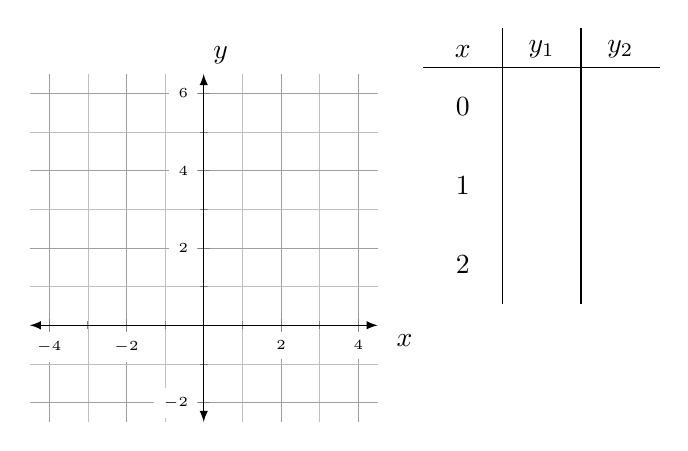
\begin{tikzpicture}[>=latex]
		\begin{axis}[
				    width =6cm,
			          height=6cm,
				    xmin=-4,xmax=4,
				    ymin=-2,ymax=6,
				    grid=both,
				    grid style={line width=.15pt, draw=gray!50},
				    major grid style={line width=.3pt,draw=gray!75},
				    axis lines=middle,
				    minor tick num=1,
				    enlargelimits={abs=0.5},
				    axis line style={latex-latex},
				    ticklabel style={font=\tiny,fill=white},
				    xlabel={\,\,$x$},
				    ylabel={$y$},
				    xlabel style={below right},
				    ylabel style={above right}
				]
		\end{axis}
		%%  T-Chart  %%%%%%%%
		\draw (6,5) --(6,1.5);
		\draw (7,5) --(7,1.5);
		\draw (5.5,4.5) node[above]{$x$} (6.5, 4.5) node[above]{$y_1$} (7.5, 4.5) node[above]{$y_2$};
		\draw (5, 4.5) -- (8, 4.5);
		\draw (5.5, 4) node{$0$};
		\draw (5.5, 3) node{$1$};
		\draw (5.5, 2) node{$2$};
		%%%%%%%%%%%%%%%
	\end{tikzpicture}
	\begin{itemize}
   	        \item[(c)] 
	        $\begin{cases}
	            x+y=4 \\
	            2y+4=x
	        \end{cases}$\\
	\end{itemize}    
\hspace{-0.5cm}
    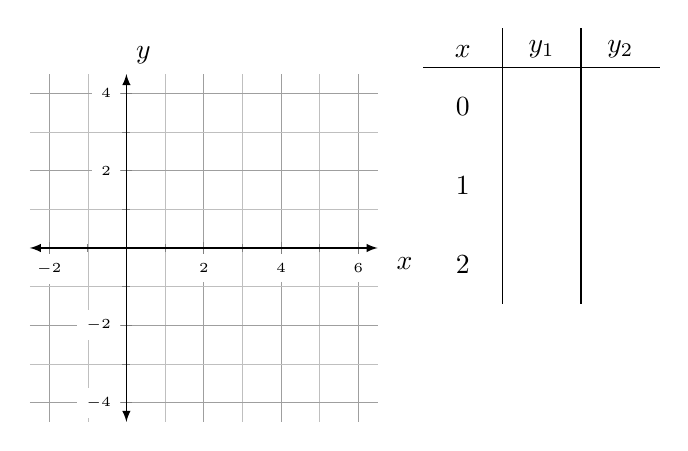
\begin{tikzpicture}[>=latex]
		\begin{axis}[
				    width =6cm,
			        height=6cm,
				    xmin=-2,xmax=6,
				    ymin=-4,ymax=4,
				    grid=both,
				    grid style={line width=.15pt, draw=gray!50},
				    major grid style={line width=.3pt,draw=gray!75},
				    axis lines=middle,
				    minor tick num=1,
				    enlargelimits={abs=0.5},
				    axis line style={latex-latex},
				    ticklabel style={font=\tiny,fill=white},
				    xlabel={\,\,$x$},
				    ylabel={$y$},
				    xlabel style={below right},
				    ylabel style={above right}
				]
		\end{axis}
		%%  T-Chart  %%%%%%%%
		\draw (6,5) --(6,1.5);
		\draw (7,5) --(7,1.5);
		\draw (5.5,4.5) node[above]{$x$} (6.5, 4.5) node[above]{$y_1$} (7.5, 4.5) node[above]{$y_2$};
		\draw (5, 4.5) -- (8, 4.5);
		\draw (5.5, 4) node{$0$};
		\draw (5.5, 3) node{$1$};
		\draw (5.5, 2) node{$2$};
		%%%%%%%%%%%%%%%
	\end{tikzpicture}
\vspace{1cm}
\end{minipage}
\hspace{1cm}
\begin{minipage}{0.35\linewidth}
\begin{itemize}
    \item[(b)] 
        $\begin{cases}
            2y+6=x \\
            4x=3+y
        \end{cases}$\\
\end{itemize}    
\hspace{-0.5cm}
    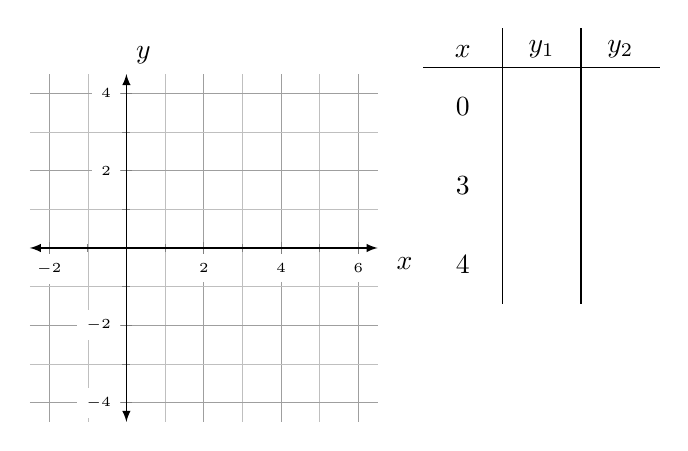
\begin{tikzpicture}[>=latex]
		\begin{axis}[
				    width =6cm,
			        height=6cm,
				    xmin=-2,xmax=6,
				    ymin=-4,ymax=4,
				    grid=both,
				    grid style={line width=.15pt, draw=gray!50},
				    major grid style={line width=.3pt,draw=gray!75},
				    axis lines=middle,
				    minor tick num=1,
				    enlargelimits={abs=0.5},
				    axis line style={latex-latex},
				    ticklabel style={font=\tiny,fill=white},
				    xlabel={\,\,$x$},
				    ylabel={$y$},
				    xlabel style={below right},
				    ylabel style={above right}
				]
		\end{axis}
		%%  T-Chart  %%%%%%%%
		\draw (6,5) --(6,1.5);
		\draw (7,5) --(7,1.5);
		\draw (5.5,4.5) node[above]{$x$} (6.5, 4.5) node[above]{$y_1$} (7.5, 4.5) node[above]{$y_2$};
		\draw (5, 4.5) -- (8, 4.5);
		\draw (5.5, 4) node{$0$};
		\draw (5.5, 3) node{$3$};
		\draw (5.5, 2) node{$4$};
		%%%%%%%%%%%%%%%
	\end{tikzpicture}
\begin{itemize}
    \item[(d)] 
        $\begin{cases}
            x+y=-7 \\
            2x-y=4
        \end{cases}$\\
\end{itemize}    
\hspace{-0.5cm}
    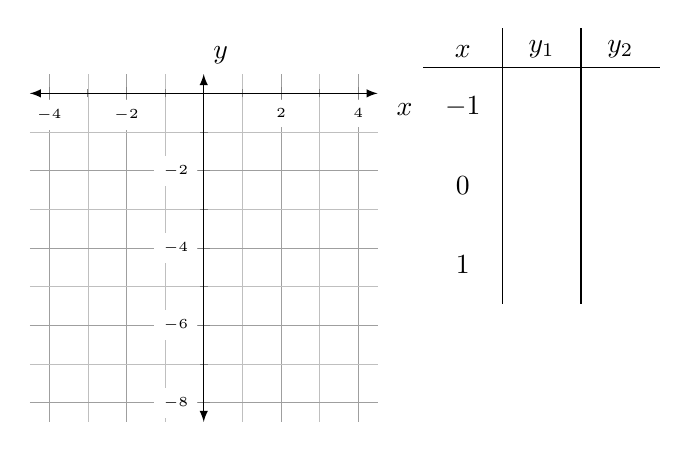
\begin{tikzpicture}[>=latex]
		\begin{axis}[
				    width =6cm,
			        height=6cm,
				    xmin=-4,xmax=4,
				    ymin=-8,ymax=0,
				    grid=both,
				    grid style={line width=.15pt, draw=gray!50},
				    major grid style={line width=.3pt,draw=gray!75},
				    axis lines=middle,
				    minor tick num=1,
				    enlargelimits={abs=0.5},
				    axis line style={latex-latex},
				    ticklabel style={font=\tiny,fill=white},
				    xlabel={\,\,$x$},
				    ylabel={$y$},
				    xlabel style={below right},
				    ylabel style={above right}
				]
		\end{axis}
		%%  T-Chart  %%%%%%%%
		\draw (6,5) --(6,1.5);
		\draw (7,5) --(7,1.5);
		\draw (5.5,4.5) node[above]{$x$} (6.5, 4.5) node[above]{$y_1$} (7.5, 4.5) node[above]{$y_2$};
		\draw (5, 4.5) -- (8, 4.5);
		\draw (5.5, 4) node{$-1$};
		\draw (5.5, 3) node{$0$};
		\draw (5.5, 2) node{$1$};
		%%%%%%%%%%%%%%%
	\end{tikzpicture}
\vspace{1cm}
\end{minipage}


%%%%%%%%%%%  SOLUTIONS  %%%%%%%%%%%%%%%%%%%
%\indent
%\vfill
%\color{red}
%
%\hspace{-0.95cm}
%\begin{flushright}
%\noindent \rotatebox[origin=c]{180}{ \underline{Solutions}}
%\end{flushright}
%
%\color{black}
%
%%%%%%%%%%  HOMEWROK   %%%%%%%%%%%%%%%%%%%


\noindent\large\fbox{ \textbf{3.1 (day 1) Homework}: page 186 \, 2-9 all, 15-21 odd. \small}

%%%%%%%%%%%%%%%%%%%%%%%%%%%%%%%%%%%%%%%%%%

%%%%%%%%%%%%%%%%%%%%%%%%%%%%%%%%%%%%%
%%%%%%%%%%%%%%%%%%%%%%%%%%%%%%%%%%%%%
\newpage
%%%%%%%%%%%%%%%%%%%%%%%%%%%%%%%%%%%%%
%%%%%%%%%%%%%%%%%%%%%%%%%%%%%%%%%%%%%


\begin{definition}
A \textbf{consistent system} is a set of equations that has at least one solution. An \textbf{inconsistent system} is a set of equations with no solutions.
\end{definition}

\hspace{-0.75cm}
\begin{minipage}{0.3\linewidth}
\begin{center}
\large \textbf{\color{blue} Exactly One\\ Solution}\color{black}\small\\
\end{center}
    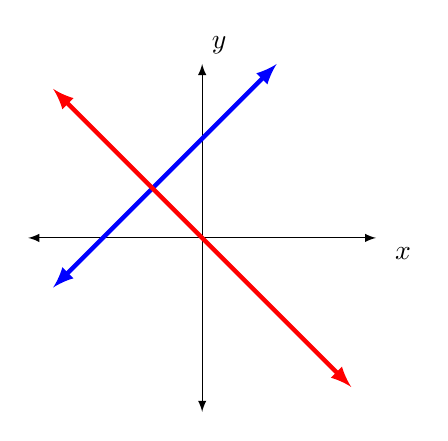
\begin{tikzpicture}[>=latex]
		\begin{axis}[
				    width =6cm,
			       	    height=6cm,
				    xmin=-3,xmax=3,
				    ymin=-3,ymax=3,
				    xticklabels={,,},
				    xtick style={draw=none},
				    yticklabels={,,},
				    ytick style={draw=none},
				    grid=none,
				    axis lines=middle,
				    enlargelimits={abs=0.5},
				    axis line style={latex-latex},
				    xlabel={\,\,$x$},
				    ylabel={$y$},
				    xlabel style={below right},
				    ylabel style={above right}
				]
    		\addplot[domain=-3:1.5, blue, ultra thick, <->] {x+2};
    		\addplot[domain=-3:3, red, ultra thick, <->] {-x};
		\end{axis}
	\end{tikzpicture}
Consistent system. The graphs are intersecting lines with different slopes.
\end{minipage}
\hspace{0.5cm}
\begin{minipage}{0.3\linewidth}
\begin{center}
\large \textbf{\color{blue} Infinitely Many\\ Solutions}\color{black}\small\\
\end{center}
    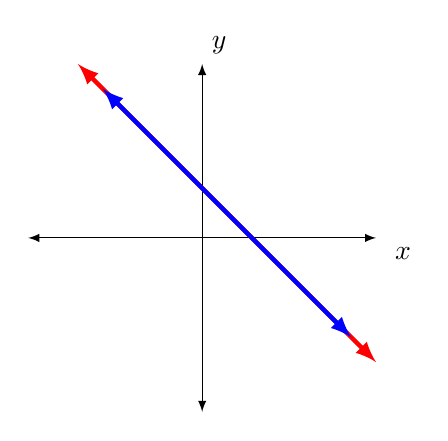
\begin{tikzpicture}[>=latex]
		\begin{axis}[
				    width =6cm,
			       	    height=6cm,
				    xmin=-3,xmax=3,
				    ymin=-3,ymax=3,
				    xticklabels={,,},
				    xtick style={draw=none},
				    yticklabels={,,},
				    ytick style={draw=none},
				    grid=none,
				    axis lines=middle,
				    enlargelimits={abs=0.5},
				    axis line style={latex-latex},
				    xlabel={\,\,$x$},
				    ylabel={$y$},
				    xlabel style={below right},
				    ylabel style={above right}
				]
    		\addplot[domain=-2.5:3.5, red, ultra thick, <->] {-x+1};
    		\addplot[domain=-2:3, blue,ultra thick, <->] {-x+1};
		\end{axis}
	\end{tikzpicture}
Consistent system. The graphs are coinciding lines; same slope and $y$-intercept.
\end{minipage}
\hspace{0.5cm}
\begin{minipage}{0.3\linewidth}
\begin{center}
\large \textbf{\color{blue}No\\ Solution}\color{black}\small\\
\end{center}
    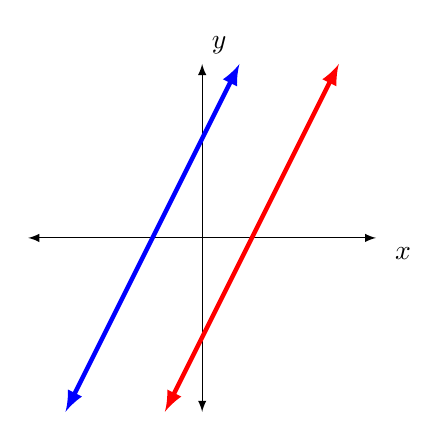
\begin{tikzpicture}[>=latex]
		\begin{axis}[
				    width =6cm,
			       	    height=6cm,
				    xmin=-3,xmax=3,
				    ymin=-3,ymax=3,
				    xticklabels={,,},
				    xtick style={draw=none},
				    yticklabels={,,},
				    ytick style={draw=none},
				    grid=none,
				    axis lines=middle,
				    enlargelimits={abs=0.5},
				    axis line style={latex-latex},
				    xlabel={\,\,$x$},
				    ylabel={$y$},
				    xlabel style={below right},
				    ylabel style={above right}
				]
    		\addplot[domain=-2.75:0.75, blue, ultra thick, <->] {2*x+2};
    		\addplot[domain=-0.75:2.75, red, ultra thick, <->] {2*x-2};
		\end{axis}
	\end{tikzpicture}
Inconsistent system. Parallel lines; same slope different $y$-intercept.
\end{minipage}

\vspace{1cm}

\begin{example}
Classify each system and determine the number of solutions.
\end{example}


\begin{minipage}{0.45\linewidth}
\begin{itemize}
    \item[(a)] 
        $\begin{cases}
            2x+y=3 \\
            6x=9-3y
        \end{cases}$\\
\end{itemize}    
\end{minipage}
\hspace{1cm}
\begin{minipage}{0.45\linewidth}
\begin{itemize}
    \item[(b)] 
        $\begin{cases}
            3x+y=3 \\
            2+y=-3x
        \end{cases}$\\
\end{itemize}    
\end{minipage}


\vspace{1cm}

\begin{minipage}{0.45\linewidth}
\begin{itemize}
    \item[(c)] 
        $\begin{cases}
            7x-y=-11 \\
            3y=21x+33
        \end{cases}$\\
\end{itemize}    
\end{minipage}
\hspace{1cm}
\begin{minipage}{0.45\linewidth}
\begin{itemize}
    \item[(d)] 
        $\begin{cases}
            x+4=y \\
            5y=5x+35
        \end{cases}$\\
\end{itemize}    
\end{minipage}

\vspace{1cm}

\begin{example}
Gavin is comparing the costs of long distance calling cards. To use card A, it costs $\$0.50$ to connect and then $\$0.05$ per minute.  To use card B, it costs $\$0.20$ to connect and then $\$0.08$ per minute. For what number of minutes does it cost the same amount to use each card for a single call?
\end{example}
\begin{flushright}
\begin{tikzpicture}
		%%  T-Chart  %%%%%%%%
		\draw (6,5) --(6,1.5);
		\draw (7,5) --(7,1.5);
		\draw (5.5,4.5) node[above]{$x$} (6.5, 4.5) node[above]{$y_A$} (7.5, 4.5) node[above]{$y_B$};
		\draw (5, 4.5) -- (8, 4.5);
		\draw (5.5, 4) node{$-1$};
		\draw (5.5, 3) node{$0$};
		\draw (5.5, 2) node{$1$};
		%%%%%%%%%%%%%%%
\end{tikzpicture}
\end{flushright}
\vfill

\noindent\large\fbox{ \textbf{3.1 (day 2) Homework}: page 186 \, 10-14 all, 23-27 odd. \small}



%%%%%%%%%%%%%%%%%%%%%%%%%%%%%%%
%%%%%%%%%%%%%%%%%%%%%%%%%%%%%%%
%%%%%%%%%%%   Section 3.2   %%%%%%%%%%%%%
 \newpage
%%%%%%%%%%%%%%%%%%%%%%%%%%%%%%%
%%%%%%%%%%%%%%%%%%%%%%%%%%%%%%%
 \section{  Using Algebraic Methods to Solve Systems  }
 \setcounter{example}{0}
 \setcounter{definition}{0}
 %%%%%%%%%%%%%%%%%%%%%%%%%%%%%%%%
 %%%%%%%%%%%%%%%%%%%%%%%%%%%%%%%%
 \begin{definition}
	\textbf{Substitution} is a method used to solve systems of equations by solving an equation for one variable and substituting the resulting expression into the other equation(s). 
 \end{definition}


%%%%%%%%%%%%%%%% Example 1
\begin{example}
     Use \textbf{substitution} to solve each system of equations.
\end{example}
%
\vspace{-0.5cm}
\hspace{-0.5cm}
%
% LeftOfPage%%%%%
\begin{minipage}{0.45\linewidth}
 \begin{itemize}
     \item[(a)]
        $\begin{cases}
            y=x+2 \\
            x+y=8
        \end{cases}$\\
 \end{itemize}
%
\vspace{2.55cm}
%
 \begin{itemize}
     \item[(c)]
        $\begin{cases}
            y=2x-1 \\
            3x+2y=26
        \end{cases}$\\
 \end{itemize}
%
\vspace{2.55cm}
%
\end{minipage}
\hspace{1.5cm}
%RightOfPage%%%%%
\begin{minipage}{0.45\linewidth}
 \begin{itemize}
     \item[(b)]
        $\begin{cases}
            2x+y=6 \\
            y-8x=1
        \end{cases}$\\
 \end{itemize}
%
\vspace{2.55cm}
%
 \begin{itemize}
     \item[(d)]
        $\begin{cases}
            5x+6y=-9 \\
            2x-2=-y
        \end{cases}$\\
 \end{itemize}
%
\vspace{2.55cm}
%
\end{minipage}
%%%%%%%%%%%%%%%%%%%%%

 \begin{definition}
\textbf{Elimination} is a method used to solve a system of equations in which one variable is eliminated by adding or subtracting two equations of the system.
 \end{definition}

%%%%%%%%%%%%%%%% Example 2
\begin{example}
     Use \textbf{elimination} to solve each system of equations.
\end{example}
%
\vspace{-0.5cm}
\hspace{-0.5cm}
%
% LeftOfPage%%%%%
\begin{minipage}{0.45\linewidth}
 \begin{itemize}
     \item[(a)]
        $\begin{cases}
            2x+3y=34 \\
            4x-3y=-4
        \end{cases}$\\
 \end{itemize}
%
\vspace{2.75cm}
%
 \begin{itemize}
     \item[(c)]
        $\begin{cases}
            \quad \,\, 4x+7y=-25 \\
            -12x-7y=19
        \end{cases}$\\
 \end{itemize}
%
\vspace{2.75cm}
%
\end{minipage}
\hspace{1.5cm}
%RightOfPage%%%%%
\begin{minipage}{0.45\linewidth}
 \begin{itemize}
     \item[(b)]
        $\begin{cases}
            2x+4y=-10 \\
            3x+3y=-3
        \end{cases}$\\
 \end{itemize}
%
\vspace{2.75cm}
%
 \begin{itemize}
     \item[(d)]
        $\begin{cases}
            5x+6y=-9 \\
            2x-2=-y
        \end{cases}$\\
 \end{itemize}
%
\vspace{2.75cm}
%
\end{minipage}
%%%%%%%%%%%%%%%%%%%%%
\vfill
\noindent \fbox{\large\textbf{3.2 (day 1) Homework}: page 194 \, 3-9 odd, 15-21 odd, 29, 31 \small }


%%%%%%%%%%%%%%%%%%%%%%%%%%%%%%%%%%%%%
%%%%%%%%%%%%%%%%%%%%%%%%%%%%%%%%%%%%%
\newpage
%%%%%%%%%%%%%%%%%%%%%%%%%%%%%%%%%%%%%
%%%%%%%%%%%%%%%%%%%%%%%%%%%%%%%%%%%%%



 \begin{example}
\textbf{Classify} the system and determine the number of solutions.
 \end{example}
%
\vspace{-0.5cm}
\hspace{-0.5cm}
%
% LeftOfPage%%%%%
\begin{minipage}{0.45\linewidth}
 \begin{itemize}
     \item[(a)]
        $\begin{cases}
            2x+y=8 \\
            6x+3y=-15
        \end{cases}$\\
 \end{itemize}
%
\vspace{2.55cm}
%
 \begin{itemize}
     \item[(c)]
        $\begin{cases}
            6x+3y=-12 \\
            2x+y=-6
        \end{cases}$\\
 \end{itemize}
%
\vspace{2.55cm}
%
\end{minipage}
\hspace{1.5cm}
%RightOfPage%%%%%
\begin{minipage}{0.45\linewidth}
 \begin{itemize}
     \item[(b)]
        $\begin{cases}
            56x+8y=-32 \\
            7x+y=-4
        \end{cases}$\\
 \end{itemize}
%
\vspace{2.55cm}
%
 \begin{itemize}
     \item[(d)]
        $\begin{cases}
            5x-y=-3 \\
            15x-3y=-9
        \end{cases}$\\
 \end{itemize}
%
\vspace{2.55cm}
%
\end{minipage}
%%%%%%%%%%%%%%%%%%%%%

%%%%%%%%%%%%%%%% Example 2
\begin{example}
Hendrix, a zookeeper, needs to mix feed for the prairie dogs so that the feed has the right amount of protein. Feed \textbf{A} has $12\%$ protein. Feed \textbf{B} has $5\%$ protein. How many pounds of each does he need to mix to get 100 lb of feed that has $8\%$ protein?
\end{example} 
%%%%%%%%%%%%%%%%%%%%
\vfill

%%%%%%%%%%%%%%%% Example 3
\begin{example}
A coffee blend contains Sumatra beans, which cost $\$5/$lb, and Kona beans, which cost $\$13/$lb. If the blend costs $\$10/$lb, how much of each type of coffee is in $50$ lb of the blend? 
\end{example}
%%%%%%%%%%%%%%%%%%%%
\vfill



 \noindent\fbox{\large\textbf{3.2 (day 2) Homework}: page 194 \, 11, 13, 14, 23, 25, 27, 29, 31 \small }



%%%%%%%%%%%%%%%%%%%%%%%%%%%%%%%
%%%%%%%%%%%%%%%%%%%%%%%%%%%%%%%
%%%%%%   Section 3.3   %%%%%%%%
%%%%%%%%%%%%%%%%%%%%%%%%%%%%%%%
%%%%%%%%%%%%%%%%%%%%%%%%%%%%%%%
 \section{Solving Systems of Linear Inequalities}
 \setcounter{example}{0}
 \setcounter{definition}{0}
 %%%%%%%%%%%%%%%%%%%%%%%%%%%%%%%%
 %%%%%%%%%%%%%%%%%%%%%%%%%%%%%%%%
\begin{definition}
	A \textbf{system of linear inequalities} is a set of two or more linear inequalities with the same variables. The \textbf{solution to a system of linear inequalities} is often an infinite set of points that can be represented graphically by shading.
\end{definition}
\begin{example}
Graph each system of inequalities.
\end{example}

\hspace{-0.5cm}
\begin{minipage}{0.45\linewidth}
	\begin{itemize}
    		\item[(a)] 
        	$\begin{cases}
            		y\leq -2x+4 \\
            		y>x-3    
        	\end{cases}$\\ 
	\end{itemize}
\hspace{-0.5cm}
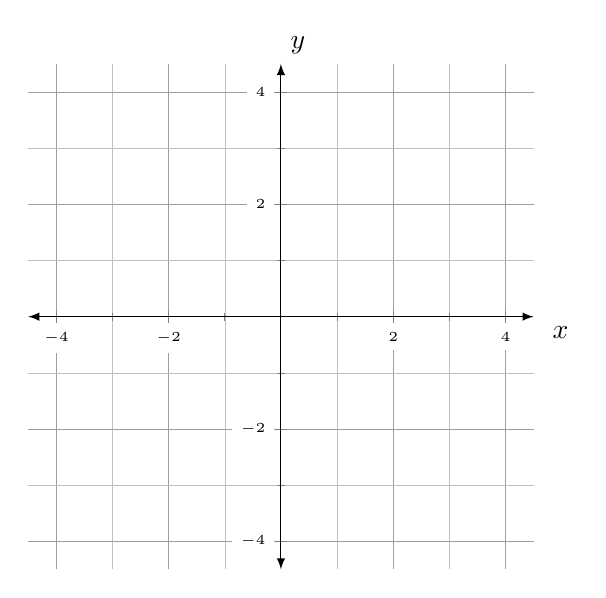
\begin{tikzpicture}[>=latex]
		\begin{axis}[
				    width =8cm,
			               height=8cm,
				    xmin=-4,xmax=4,
				    ymin=-4,ymax=4,
				    grid=both,
				    grid style={line width=.15pt, draw=gray!50},
				    major grid style={line width=.3pt,draw=gray!75},
				    axis lines=middle,
				    minor tick num=1,
				    enlargelimits={abs=0.5},
				    axis line style={latex-latex},
				    ticklabel style={font=\tiny,fill=white},
				    xlabel={\,\,$x$},
				    ylabel={$y$},
				    xlabel style={below right},
				    ylabel style={above right}
				]
		\end{axis}
\end{tikzpicture}
%
\vspace{1.5cm}
%
\begin{itemize}
   	     \item[(c)] 
	     $\begin{cases}
	            x-3y<6 \\
	            2x+y>1.5
	    \end{cases}$\\
\end{itemize}    
\hspace{-0.5cm}
    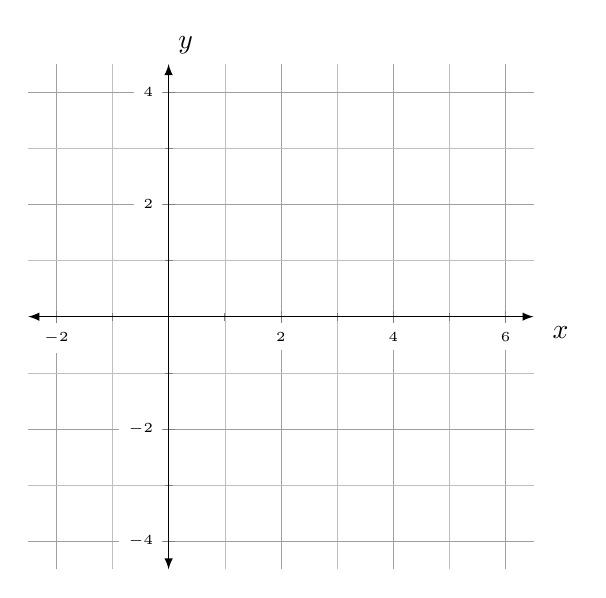
\begin{tikzpicture}[>=latex]
		\begin{axis}[
				    width =8cm,
			               height=8cm,
				    xmin=-2,xmax=6,
				    ymin=-4,ymax=4,
				    grid=both,
				    grid style={line width=.15pt, draw=gray!50},
				    major grid style={line width=.3pt,draw=gray!75},
				    axis lines=middle,
				    minor tick num=1,
				    enlargelimits={abs=0.5},
				    axis line style={latex-latex},
				    ticklabel style={font=\tiny,fill=white},
				    xlabel={\,\,$x$},
				    ylabel={$y$},
				    xlabel style={below right},
				    ylabel style={above right}
				]
		\end{axis}
	\end{tikzpicture}
\end{minipage}
\hspace{1cm}
\begin{minipage}{0.35\linewidth}
\begin{itemize}
    \item[(b)] 
        $\begin{cases}
            y\geq \displaystyle\frac{3}{2}x+2 \\
            x<3
        \end{cases}$\\
\end{itemize}    
\hspace{-0.5cm}
    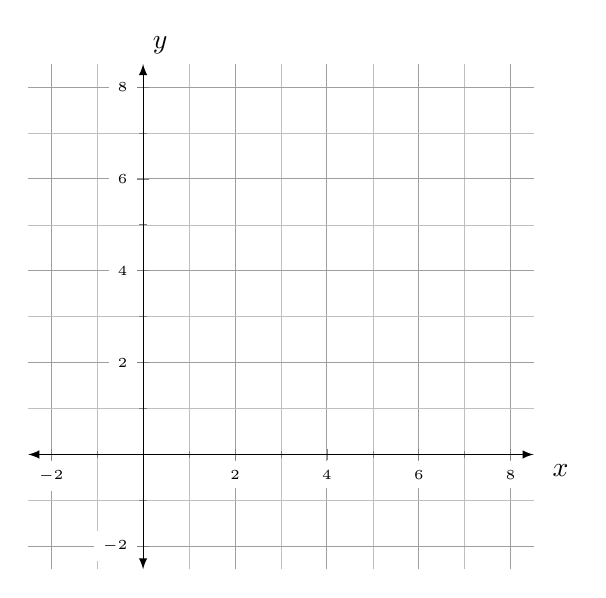
\begin{tikzpicture}[>=latex]
		\begin{axis}[
				    width =8cm,
			        	    height=8cm,
				    xmin=-2,xmax=8,
				    ymin=-2,ymax=8,
				    grid=both,
				    grid style={line width=.15pt, draw=gray!50},
				    major grid style={line width=.3pt,draw=gray!75},
				    axis lines=middle,
				    minor tick num=1,
				    enlargelimits={abs=0.5},
				    axis line style={latex-latex},
				    ticklabel style={font=\tiny,fill=white},
				    xlabel={\,\,$x$},
				    ylabel={$y$},
				    xlabel style={below right},
				    ylabel style={above right}
				]
		\end{axis}
	\end{tikzpicture}
%
\vspace{1cm}
%
\begin{itemize}
    \item[(d)] 
        $\begin{cases}
            y\leq 4 \\
            2x+y<1
        \end{cases}$\\
\end{itemize}    
\hspace{-0.5cm}
    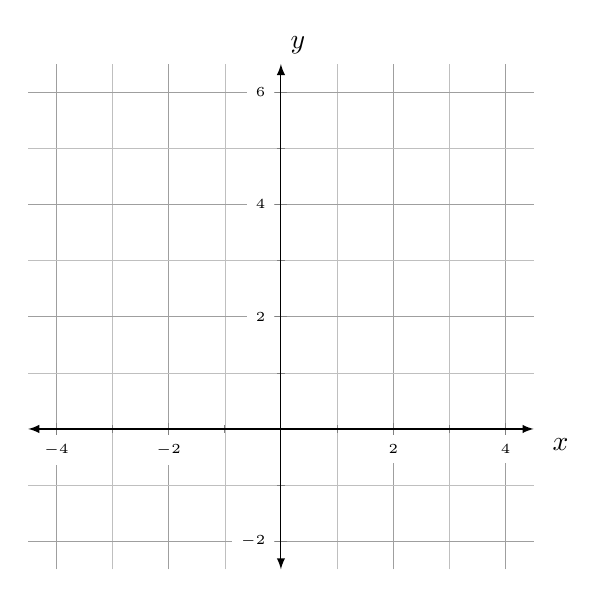
\begin{tikzpicture}[>=latex]
		\begin{axis}[
				    width =8cm,
			       	    height=8cm,
				    xmin=-4,xmax=4,
				    ymin=-2,ymax=6,
				    grid=both,
				    grid style={line width=.15pt, draw=gray!50},
				    major grid style={line width=.3pt,draw=gray!75},
				    axis lines=middle,
				    minor tick num=1,
				    enlargelimits={abs=0.5},
				    axis line style={latex-latex},
				    ticklabel style={font=\tiny,fill=white},
				    xlabel={\,\,$x$},
				    ylabel={$y$},
				    xlabel style={below right},
				    ylabel style={above right}
				]
		\end{axis}
	\end{tikzpicture}
\end{minipage}
\vfill

%%%%%%%%%%%%%%%%%%%%%%%%%%%%%%%%%%%%%
%%%%%%%%%%%%%%%%%%%%%%%%%%%%%%%%%%%%%
 \newpage
%%%%%%%%%%%%%%%%%%%%%%%%%%%%%%%%%%%%%
%%%%%%%%%%%%%%%%%%%%%%%%%%%%%%%%%%%%%

\begin{example}
Brayden leads a polar expedition 240 miles away from camp, and a snowstorm will reach the camp in 48 hours. The expedition will travel as far as possible by boat and then walk the remaining distance. Brayden and his men can navigate by boat 12 miles per hour and walk at a rate of 3 miles per hour. Write and graph a system of inequalities that can be used to determine how long the explorers may travel by foot or by boat to reach their camp before the storm. 
\end{example}

\begin{flushright}
    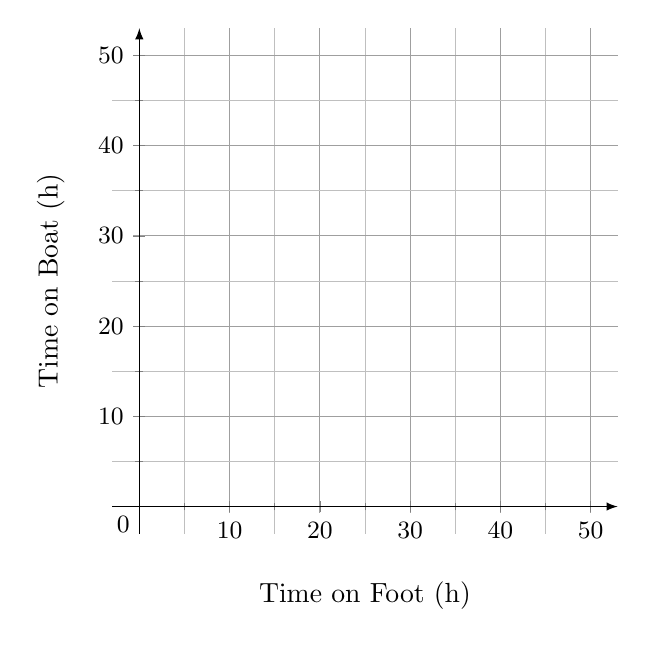
\begin{tikzpicture}
		\begin{axis}[
				    width =8cm,
			       	    height=8cm,
				    xmin=0,xmax=50,
				    ymin=0,ymax=50,
				    grid=both,
				    grid style={line width=.15pt, draw=gray!50},
				    major grid style={line width=.3pt,draw=gray!75},
				    axis lines=middle,
				    minor tick num=1,
				    enlargelimits={abs=3},
				    axis line style={-latex},
				    ticklabel style={font=\small,fill=white},
				    xlabel={Time on Foot (h)},
				    ylabel={Time on Boat (h)},
				    x label style={at={(axis description cs:0.5,-0.075)},anchor=north},
				    y label style={at={(axis description cs:-0.075,.5)},rotate=90,anchor=south},
				]
			  \node[below left] at (axis cs:0,0) {\small$0$};
		\end{axis}
	\end{tikzpicture}
\end{flushright}

\begin{example}
Ryan is selling hot dogs and spicy sausages at the fair. He has only 40 buns, so he can sell no more than a total of 40 hot dogs and sausages. Each hot dog sells for $\$2$, and each sausage sells for $\$2.50$. Ryan needs at least $\$90$ in sales to meet his goal. Write and graph a system of inequalities that models the situation.
\end{example}

\begin{flushright}
    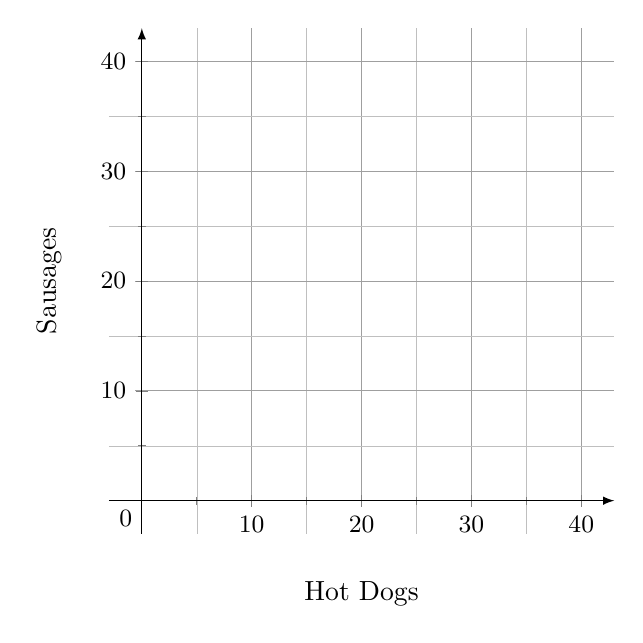
\begin{tikzpicture}
		\begin{axis}[
				    width =8cm,
			       	    height=8cm,
				    xmin=0,xmax=40,
				    ymin=0,ymax=40,
				    grid=both,
				    grid style={line width=.15pt, draw=gray!50},
				    major grid style={line width=.3pt,draw=gray!75},
				    axis lines=middle,
				    minor tick num=1,
				    enlargelimits={abs=3},
				    axis line style={-latex},
				    ticklabel style={font=\small,fill=white},
				    xlabel={Hot Dogs},
				    ylabel={Sausages},
				    x label style={at={(axis description cs:0.5,-0.075)},anchor=north},
				    y label style={at={(axis description cs:-0.075,.5)},rotate=90,anchor=south},
				]
			  \node[below left] at (axis cs:0,0) {\small$0$};
		\end{axis}
	\end{tikzpicture}
\end{flushright}





 \noindent\fbox{\large\textbf{3.3 Homework}: page 202 \, 1-8 all,   \small }
%%%%%%%%%%%%%%%%%%%%%%%%%%%%%%%%%%%%%
%%%%%%%%%%%%%%%%%%%%%%%%%%%%%%%%%%%%%
 \newpage
%%%%%%%%%%%%%%%%%%%%%%%%%%%%%%%%%%%%%
%%%%%%%%%%%%%%%%%%%%%%%%%%%%%%%%%%%%%

%%%%%%%%%%%%%%%%%%%%%%%%%%%%%%%
%%%%%%%%%%%%%%%%%%%%%%%%%%%%%%%
%%%%%%   Section 3.4   %%%%%%%%
%%%%%%%%%%%%%%%%%%%%%%%%%%%%%%%
%%%%%%%%%%%%%%%%%%%%%%%%%%%%%%%
 \section{   Linear Programming  }
 \setcounter{example}{0}
 \setcounter{definition}{0}
 %%%%%%%%%%%%%%%%%%%%%%%%%%%%%%%%
 %%%%%%%%%%%%%%%%%%%%%%%%%%%%%%%%
 \begin{definition}
 \textbf{Linear Programming} is a method of finding a maximum or minimum value of a function that satisfies a given set of conditions called \emph{constraints}. A \textbf{constraint} is one of the inequalities in a linear programming problem. The solution to the set of constraints can be graphed as a \textbf{feasible (or bounded) region}. 
 \end{definition}

%%%%%%%%%%%%%%%% Example 1
\begin{example}
Graph the feasible region for the following constraints.
\end{example}

$
\begin{cases}
x\geq 0\\
y\geq 1.5\\
2.5x+5y\leq20\\
3x+2y\leq12
\end{cases}
$

\vspace{-3.5cm}
\begin{flushright}
    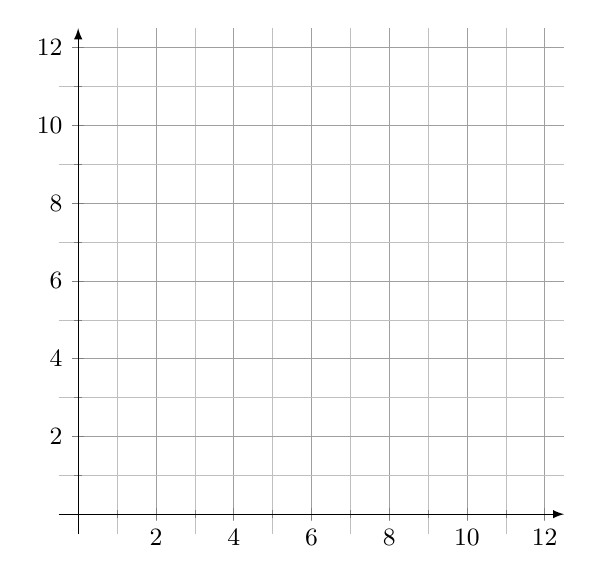
\begin{tikzpicture}
		\begin{axis}[
				    width =8cm,
			       	    height=8cm,
				    xmin=0,xmax=12,
				    ymin=0,ymax=12,
				    grid=both,
				    grid style={line width=.15pt, draw=gray!50},
				    major grid style={line width=.3pt,draw=gray!75},
				    axis lines=middle,
				    minor tick num=1,
				    enlargelimits={abs=0.5},
				    axis line style={-latex},
				    ticklabel style={font=\small,fill=white},
				]
		\end{axis}
	\end{tikzpicture}
\end{flushright}

%%%%%%%%%%%%%%%%%%%% Example 2

 \begin{example}
Rileigh is planning a green roof that will cover up to 600 sqare feet. She will use two types of plants: blue lagoon sedum and raspberry red sedum. Each blue lagoon sedum will cover 1.2 square feet. Each raspberry red sedum will cover 2 square feet. Each plant costs $\$ 2.50$, and Rileigh must spend less than $\$1000$. Write the constraints, and graph the feasible region.
 \end{example}

\begin{flushright}
    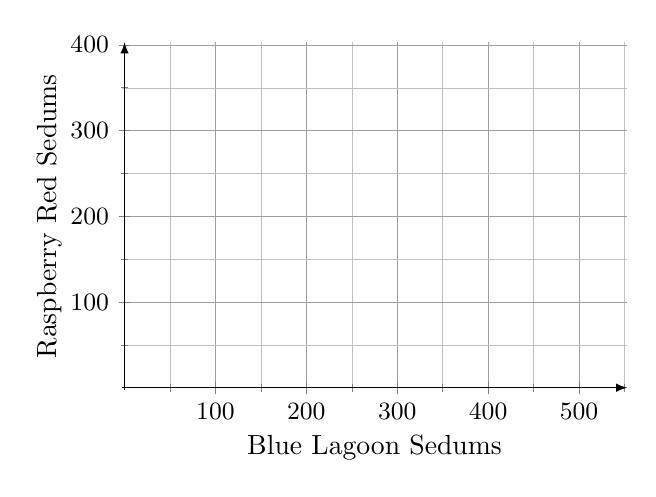
\begin{tikzpicture}
		\begin{axis}[
				    width =8cm,
			       	    height=6cm,
				    xmin=0,xmax=550,
				    ymin=0,ymax=400,
				    grid=both,
				    grid style={line width=.15pt, draw=gray!50},
				    major grid style={line width=.3pt,draw=gray!75},
				    axis lines=middle,
				    minor tick num=1,
				    enlargelimits={abs=3},
				    axis line style={-latex},
				    ticklabel style={font=\small,fill=white},
				    xlabel={Blue Lagoon Sedums},
				    ylabel={Raspberry Red Sedums},
				    x label style={at={(axis description cs:0.5,-0.1)},anchor=north},
				    y label style={at={(axis description cs:-0.1,.5)},rotate=90,anchor=south},
				]
			  \node[below left] at (axis cs:0,0) {\small$0$};
		\end{axis}
	\end{tikzpicture}
\end{flushright}

%%%%%%%%%%%%%%%%%%%%%

\begin{definition} 
In most linear programming problems, you want to do more than identify the feasible region. Often you want to find the best combination of values in order to minimize or maximize a certain function. This function is the \textbf{objective function}. If an objective function (of a linear program) has a maximum or minimum value, it must occur at one or more of the vertices of a feasible region.
\end{definition}




%%%%%%%%%%%%%%%%%%%%%%%%%%%%%%%%%%%%%
%%%%%%%%%%%%%%%%%%%%%%%%%%%%%%%%%%%%%
 \newpage
%%%%%%%%%%%%%%%%%%%%%%%%%%%%%%%%%%%%%
%%%%%%%%%%%%%%%%%%%%%%%%%%%%%%%%%%%%%



%%%%%%%%%%%%%%%%%%%% Example 3
\begin{example}
One of Rileigh's priorities for the green roof is to help control air pollution. To do this, she wants to maximize the amount of carbon dioxide the plants on the roof can absorb. If the blue lagoon sedum can absorb 1.4 lbs of $\text{CO}_2$ per year and the red raspberry, 2.1 lbs per year. Find the number of each plant Rileigh should plant to maximize $\text{CO}_2$ consumption.
\end{example}

\vfill

%%%%%%%%%%%%%%%%%%%% Example 4
\begin{example}
Maximize the objective function $P=25x+30y$ under the following constraints (from \textbf{Example 1}).
\end{example}

$
\begin{cases}
x\geq 0\\
y\geq 1.5\\
2.5x+5y\leq20\\
3x+2y\leq12
\end{cases}
$




\vfill
 \noindent\fbox{\large\textbf{3.4 Homework}: page 209 \, 1, 2, 3, 5, 6, 8 \small }

%%%%%%%%%%%%%%%%%%%%%%%%%%%%%%%%%%%%%
%%%%%%%%%%%%%%%%%%%%%%%%%%%%%%%%%%%%%
 \newpage
%%%%%%%%%%%%%%%%%%%%%%%%%%%%%%%%%%%%%
%%%%%%%%%%%%%%%%%%%%%%%%%%%%%%%%%%%%%


%%%%%%%%%%%%%%%%%%%%%%%%%%%%%%%
%%%%%%%%%%%%%%%%%%%%%%%%%%%%%%%
%%%%%%   Section 3.5   %%%%%%%%
%%%%%%%%%%%%%%%%%%%%%%%%%%%%%%%
%%%%%%%%%%%%%%%%%%%%%%%%%%%%%%%
 \section{    Linear Equations in Three Dimensions   }
 \setcounter{example}{0}
 \setcounter{definition}{0}
 %%%%%%%%%%%%%%%%%%%%%%%%%%%%%%%%
 %%%%%%%%%%%%%%%%%%%%%%%%%%%%%%%%

\vspace{-1cm}

\begin{minipage}{0.45\linewidth}
 \begin{definition}
 You can represent any location in three-dimensional space using\newline a \textbf{three-dimensional coordinate system}, sometimes called \emph{coordinate space}
 \end{definition}
\vspace{0.25cm}
\begin{definition}
Each point in coordinate space can be represented by an \textbf{ordered triple} of the form $(x,y,z)$. The system is similar to the coordinate plane but has an additional coordinate based on the $z$-axis. Notice the the axes form three planes that intersect at the origin $(0,0,0)$.
\end{definition}
\end{minipage}
\hfill
\begin{minipage}{0.45\linewidth}
%%%%%%%%%%%%% 3 Space Sample
\begin{flushright}
	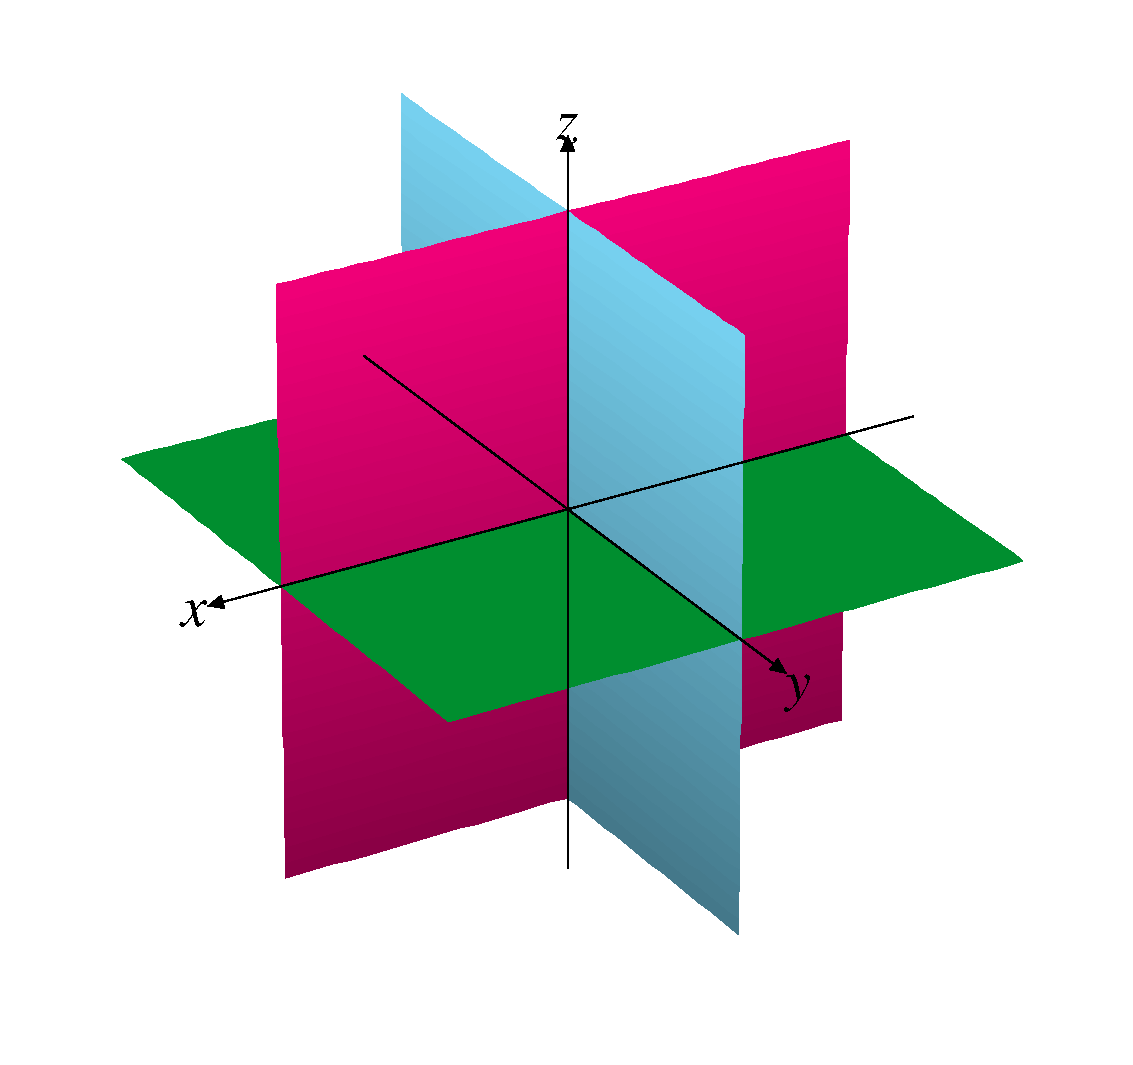
\includegraphics[scale=0.45]{3space.eps}
\end{flushright}
%%%%%%%%%%%%%%%%%
\end{minipage}


%%%%%%%%%%%%%%%%%%%%%%%%%Example 1
 \begin{example}
 Graph each point in three-dimensional space using the axes provided.
 \end{example}


\begin{minipage}{0.45\linewidth}
\vspace{-3cm}
 \begin{itemize}
	\item[(a)] A$(2,3,-2)$
	%
	\vspace{1cm}
	%
	\item[(b)] B$(-1,1,2)$
	%
	\vspace{1cm}
	%
	\item[(c)] C$(-3,-3,0)$
\end{itemize}
\end{minipage}
\hfill
\begin{minipage}{0.45\linewidth}
\vspace{-0.75cm}
\begin{flushright}
%%%%%%%%%%%%%%%%% 3space Axes to Plot On
\begin{tikzpicture}[x=0.5cm,y=0.5cm,z=0.3cm,>=latex,scale=1.25]
% The axes
\draw[->] (xyz cs:x=-5.5) -- (xyz cs:x=5.5) node[above] {$y$};
\draw[->] (xyz cs:y=-5.5) -- (xyz cs:y=5.5) node[right] {$z$};
\draw[<-] (xyz cs:z=-5.5) node[above] {$x$} -- (xyz cs:z=5.5);
% The thin ticks
\foreach \coo in {-5,-4,...,5}
{
  \draw (\coo,-1.5pt) -- (\coo,1.5pt);
  \draw (-1.5pt,\coo) -- (1.5pt,\coo);
  \draw (xyz cs:y=-0.15pt,z=\coo) -- (xyz cs:y=0.15pt,z=\coo);
}
% The thick ticks
\foreach \coo in {5,-5}
{
  \draw[thick] (\coo,-3pt)  node[below]{\coo} -- (\coo,3pt) ;
  \draw[thick] (-3pt,\coo) -- (3pt,\coo) node[left=6pt] {\coo};
  \draw[thick] (xyz cs:y=-0.3pt,z=-\coo) -- (xyz cs:y=0.3pt,z=-\coo) node[below=8pt] {\coo};
}
\end{tikzpicture}
%%%%%%%%%%%%%%%%%
\end{flushright}
\end{minipage}


%%%%%%%%%%%%%%%%%%%%%%%%%Example 2
 \begin{example}
Graph the linear equation $3x+4y+2z=12$ in three-dimensional space.
 \end{example}

\vspace{-0.75cm}
\begin{flushright}
%%%%%%%%%%%%%%%%% 3space Axes to Plot On
\begin{tikzpicture}[x=0.5cm,y=0.5cm,z=0.3cm,>=latex,scale=1.25]
% The axes
\draw[->] (xyz cs:x=-5.5) -- (xyz cs:x=5.5) node[above] {$y$};
\draw[->] (xyz cs:y=-5.5) -- (xyz cs:y=5.5) node[right] {$z$};
\draw[<-] (xyz cs:z=-5.5) node[above] {$x$} -- (xyz cs:z=5.5);
% The thin ticks
\foreach \coo in {-5,-4,...,5}
{
  \draw (\coo,-1.5pt) -- (\coo,1.5pt);
  \draw (-1.5pt,\coo) -- (1.5pt,\coo);
  \draw (xyz cs:y=-0.15pt,z=\coo) -- (xyz cs:y=0.15pt,z=\coo);
}
% The thick ticks
\foreach \coo in {5,-5}
{
  \draw[thick] (\coo,-3pt)  node[below]{\coo} -- (\coo,3pt) ;
  \draw[thick] (-3pt,\coo) -- (3pt,\coo) node[left=6pt] {\coo};
  \draw[thick] (xyz cs:y=-0.3pt,z=-\coo) -- (xyz cs:y=0.3pt,z=-\coo) node[below=8pt] {\coo};
}
\end{tikzpicture}
%%%%%%%%%%%%%%%%%
\end{flushright}


%%%%%%%%%%%%%%%%%%%%%%%%%%%%%%%%%%%%%
%%%%%%%%%%%%%%%%%%%%%%%%%%%%%%%%%%%%%
 \newpage
%%%%%%%%%%%%%%%%%%%%%%%%%%%%%%%%%%%%%
%%%%%%%%%%%%%%%%%%%%%%%%%%%%%%%%%%%%%


%%%%%%%%%%%%%%%%%%%%%%%%%Example 3
 \begin{example}
Graph the linear equation $x-4y+2z=4$ in three-dimensional space.
 \end{example}

\vspace{-0.75cm}
\begin{flushright}
%%%%%%%%%%%%%%%%% 3space Axes to Plot On
\begin{tikzpicture}[x=0.5cm,y=0.5cm,z=0.3cm,>=latex,scale=1.25]
% The axes
\draw[->] (xyz cs:x=-5.5) -- (xyz cs:x=5.5) node[above] {$y$};
\draw[->] (xyz cs:y=-5.5) -- (xyz cs:y=5.5) node[right] {$z$};
\draw[<-] (xyz cs:z=-5.5) node[above] {$x$} -- (xyz cs:z=5.5);
% The thin ticks
\foreach \coo in {-5,-4,...,5}
{
  \draw (\coo,-1.5pt) -- (\coo,1.5pt);
  \draw (-1.5pt,\coo) -- (1.5pt,\coo);
  \draw (xyz cs:y=-0.15pt,z=\coo) -- (xyz cs:y=0.15pt,z=\coo);
}
% The thick ticks
\foreach \coo in {5,-5}
{
  \draw[thick] (\coo,-3pt)  node[below]{\coo} -- (\coo,3pt) ;
  \draw[thick] (-3pt,\coo) -- (3pt,\coo) node[left=6pt] {\coo};
  \draw[thick] (xyz cs:y=-0.3pt,z=-\coo) -- (xyz cs:y=0.3pt,z=-\coo) node[below=8pt] {\coo};
}
\end{tikzpicture}
%%%%%%%%%%%%%%%%%
\end{flushright}


%%%%%%%%%%%%%%%%%%%%%%%% Example 4
\begin{example}
A computer game uses a role-playing scenario in which players build civilizations. Each player begins with 100 gold coins to buy resources. The players then compete for the survival of their civilizations. Each unit of food costs 2 gold, wood costs 4 gold, and stone costs 5 gold.
\end{example}

\begin{itemize}
\item[(a)] Write a linear equation in three variables to model this situation. 
\end{itemize}

\vfill
\begin{itemize}
\item[(b)] Use the table to find the number of units of stone each player can buy. 
\end{itemize}

\begin{flushright}
\begin{tabular}{|l|c|c|c|}
\hline
&&&\\
&\textbf{Units}&\textbf{Units}&\textbf{Units}\\
\textbf{Player}&\textbf{of Food}&\textbf{of Wood}&\textbf{of Stone}\\
\hline
Owen&20&10&\\
\hline
Jaclyn&15&15&\\
\hline
Madelyn&40&5&\\
\hline
Abby&25&10&\\
\hline
\end{tabular}
\end{flushright}
\vfill
\vfill




\vfill
 \noindent\fbox{\large\textbf{3.5 Homework}: page 216 \, 2-9 all, 27 \small }
%%%%%%%%%%%%%%%%%%%%%%%%%%%%%%%%%%%%%
%%%%%%%%%%%%%%%%%%%%%%%%%%%%%%%%%%%%%
 \newpage
%%%%%%%%%%%%%%%%%%%%%%%%%%%%%%%%%%%%%
%%%%%%%%%%%%%%%%%%%%%%%%%%%%%%%%%%%%%

%%%%%%%%%%%%%%%%%%%%%%%%%%%%%%%
%%%%%%%%%%%%%%%%%%%%%%%%%%%%%%%
%%%%%%   Section 3.6   %%%%%%%%
%%%%%%%%%%%%%%%%%%%%%%%%%%%%%%%
%%%%%%%%%%%%%%%%%%%%%%%%%%%%%%%
 \section{  Solving Linear Systems in Three Variables  }
 \setcounter{example}{0}
 \setcounter{definition}{0}
 %%%%%%%%%%%%%%%%%%%%%%%%%%%%%%%%
 %%%%%%%%%%%%%%%%%%%%%%%%%%%%%%%%

Recall from last section that the graph of a linear equation of three variables is a plane. Supposing we have a system of such equations results in three planes that may or may not intersect. Consider each senerio below.

\vspace{-0.5cm}

\begin{center}
\fbox{\large No Solution, Inconsistent Systems \normalsize}
\end{center}

\vspace{-0.5cm}
\begin{minipage}{0.3\linewidth}
	\begin{center}
		
\includegraphics[scale=0.25]{ParallelPlanes.eps}
	\end{center}
\end{minipage}
\hfill
\begin{minipage}{0.3\linewidth}
	\begin{center}
		
\includegraphics[scale=0.25]{TransversalPlane.eps}
	\end{center}
\end{minipage}
\hfill
\begin{minipage}{0.3\linewidth}
	\begin{center}
		
\includegraphics[scale=0.25]{TrianglePlane.eps}
	\end{center}
\end{minipage}

\begin{minipage}{0.45\linewidth}
\fbox{\large One Solution, Consistent Systems \normalsize}
	\vspace{-0.25cm}
	\begin{center}
		
\includegraphics[scale=0.35]{SingleSolution.eps}
	\end{center}
\end{minipage}
\hfill 
\begin{minipage}{0.45\linewidth}
	\fbox{\large Infinite Solutions, Consistent Systems \normalsize}
	\vspace{-0.25cm}
	\begin{center}
		
\includegraphics[scale=0.35]{InfiniteSolution.eps}
	\end{center}
\end{minipage}


 \begin{example}
 Use elimination to solve the following system of equations.
 \end{example}
$
\begin{cases}
\begin{tabular}{rcrcrcr}
$x$&$+$&$2y$&$-$&$3z$&$=$&$-2$\\
$2x$&$-$&$2y$&$+$&$z$&$=$&$7$\\
$x$&$+$&$y$&$+$&$2z$&$=$&$-4$
\end{tabular}
\end{cases}
$


%%%%%%%%%%%%%%%%%%%%%%%%%%%%%%%%%%%%%
%%%%%%%%%%%%%%%%%%%%%%%%%%%%%%%%%%%%%
 \newpage
%%%%%%%%%%%%%%%%%%%%%%%%%%%%%%%%%%%%%
%%%%%%%%%%%%%%%%%%%%%%%%%%%%%%%%%%%%%

 \begin{example}
 Use elimination to solve the following system of equations.
 \end{example}
$
\begin{cases}
\begin{tabular}{rcrcrcr}
$-x$&$+$&$y$&$+$&$2z$ &$=$&$7$\\
$2x$&$+$&$3y$&$+$&$z$&$=$&$1$\\
$-3x$&$-$&$4y$&$+$&$z$&$=$&$4$
\end{tabular}
\end{cases}
$

\vfill
\vfill
 \begin{example}
Classify and determine the number of solutions.
 \end{example}
$
\begin{cases}
\begin{tabular}{rcrcrcr}
$4x$&$-$&$2y$&$+$&$4z$ &$=$&$8$\\
$-3x$&$+$&$y$&$-$&$z$&$=$&$-4$\\
$-2x$&$+$&$2y$&$-$&$6z$&$=$&$4$
\end{tabular}
\end{cases}
$


\vfill
 \begin{example}
Classify and determine the number of solutions.
 \end{example}
$
\begin{cases}
\begin{tabular}{rcrcrcr}
$3x$&$-$&$y$&$+$&$2z$ &$=$&$4$\\
$2x$&$-$&$y$&$+$&$3z$&$=$&$7$\\
$-9x$&$+$&$3y$&$-$&$6z$&$=$&$-12$
\end{tabular}
\end{cases}
$

\vfill
 \noindent\fbox{\large\textbf{3.6 Homework}: page 224 \, 1, 3, 5, 6 \small }

%%%%%%%%%%%%%%%%%%%%%%%%%%%%%%%%%%%%%
%%%%%%%%%%%%%%%%%%%%%%%%%%%%%%%%%%%%%
 \newpage
%%%%%%%%%%%%%%%%%%%%%%%%%%%%%%%%%%%%%
%%%%%%%%%%%%%%%%%%%%%%%%%%%%%%%%%%%%%

%%%%%%%%%%%%%%%%%%%%%%%%%%%%%%%
%%%%%%%%%%%%%%%%%%%%%%%%%%%%%%%
%%%%%%   Section 3.6 Extension   %%%%%%%%
%%%%%%%%%%%%%%%%%%%%%%%%%%%%%%%
%%%%%%%%%%%%%%%%%%%%%%%%%%%%%%%
\rhead{Algebra 2: Section  \getcurrentref{chapter}.Extension}
\noindent\Large\textbf{Chapter 3 Extension: Parametric Equations}\normalsize
 \setcounter{example}{0}
 \setcounter{definition}{0}
 %%%%%%%%%%%%%%%%%%%%%%%%%%%%%%%%
 %%%%%%%%%%%%%%%%%%%%%%%%%%%%%%%%
 \begin{definition}
 Rates are commonly expressed in terms of time (mi/h, km/h, m/s, ...). When two variables, such as $x$ and $y$ are expressed in terms of a third variable, such as $t$ or $s$, the third variableis called a parameter. The equations that define this relationship are called parametric equations.
 \end{definition}
 \begin{example}
 Draw a graph to represent each set of parametric equations.
 \end{example}

\vspace{-0.5cm}
\hspace{-0.5cm}
%
% LeftOfPage%%%%%
\begin{minipage}{0.45\linewidth}
\vspace{-2cm}
 \begin{itemize}
     \item[(a)]
$
\begin{cases}
x=3t\\
y=2t
\end{cases}
$
\vspace{3cm}
 \end{itemize}
%
\vspace{2.75cm}
%
 \begin{itemize}
     \item[(b)]
$
\begin{cases}
x=t-2\\
y=4-2t
\end{cases}
$
 \end{itemize}
%
\vspace{2.75cm}
%
\end{minipage}
\hspace{1.5cm}
%RightOfPage%%%%%
\begin{minipage}{0.45\linewidth}
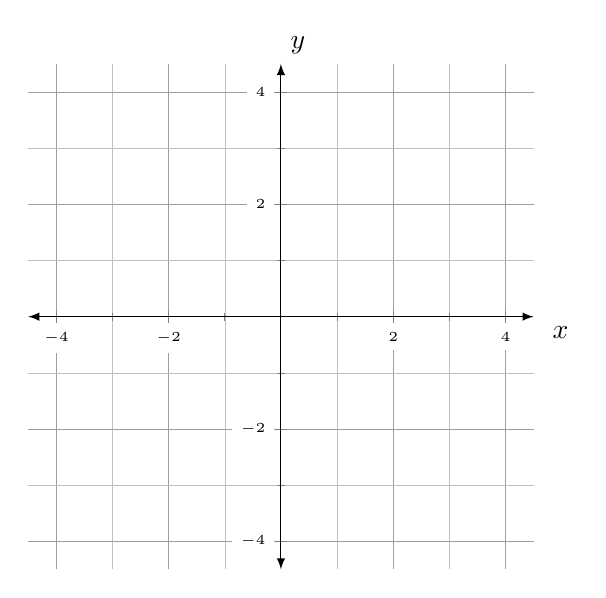
\begin{tikzpicture}[>=latex]
		\begin{axis}[
				    width =8cm,
			               height=8cm,
				    xmin=-4,xmax=4,
				    ymin=-4,ymax=4,
				    grid=both,
				    grid style={line width=.15pt, draw=gray!50},
				    major grid style={line width=.3pt,draw=gray!75},
				    axis lines=middle,
				    minor tick num=1,
				    enlargelimits={abs=0.5},
				    axis line style={latex-latex},
				    ticklabel style={font=\tiny,fill=white},
				    xlabel={\,\,$x$},
				    ylabel={$y$},
				    xlabel style={below right},
				    ylabel style={above right}
				]
		\end{axis}
\end{tikzpicture}
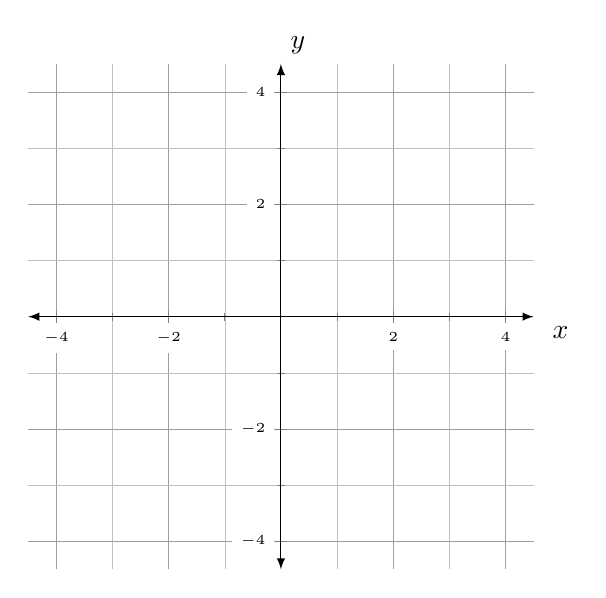
\begin{tikzpicture}[>=latex]
		\begin{axis}[
				    width =8cm,
			               height=8cm,
				    xmin=-4,xmax=4,
				    ymin=-4,ymax=4,
				    grid=both,
				    grid style={line width=.15pt, draw=gray!50},
				    major grid style={line width=.3pt,draw=gray!75},
				    axis lines=middle,
				    minor tick num=1,
				    enlargelimits={abs=0.5},
				    axis line style={latex-latex},
				    ticklabel style={font=\tiny,fill=white},
				    xlabel={\,\,$x$},
				    ylabel={$y$},
				    xlabel style={below right},
				    ylabel style={above right}
				]
		\end{axis}
\end{tikzpicture}
\end{minipage}
%%%%%%%%%%%%%%%%%%%%%

%%%%%%%%%%%%%%%% Example 2
\begin{example}
Write one parametric equation for each set of parametric equations in terms of only $x$ and $y$.
\end{example}
%
\vspace{-0.5cm}
\hspace{-0.5cm}
%
\begin{minipage}{0.45\linewidth}
 \begin{itemize}
     \item[(a)]
$
\begin{cases}
x=-4t\\
y=3t+5
\end{cases}
$
 \end{itemize}
%
\vspace{1cm}
%
 \begin{itemize}
     \item[(b)]
$
\begin{cases}
x=6t\\
y=5-2t
\end{cases}
$
 \end{itemize}
%
\vspace{1cm}
%
\end{minipage}
%%%%%%%%%%%%%%%%%%%%
\vfill
 \noindent\fbox{\large\textbf{Ch. 3 Extension Homework}: page 231 \, 1-10 all \small }
%%%%%%%%%%%%%%%%%%%%%%%%%%%%%%%%%%%%%
%%%%%%%%%%%%%%%%%%%%%%%%%%%%%%%%%%%%%
 \newpage
%%%%%%%%%%%%%%%%%%%%%%%%%%%%%%%%%%%%%
%%%%%%%%%%%%%%%%%%%%%%%%%%%%%%%%%%%%%



%%%%%%%%%%%%%%%%%%%%%%%%%%%%%%%
%%%%%%%%%%%%%%%%%%%%%%%%%%%%%%%
%%%%%%                 Chapter 3 Review                 %%%%%%%%
%%%%%%%%%%%%%%%%%%%%%%%%%%%%%%%
%%%%%%%%%%%%%%%%%%%%%%%%%%%%%%%
\rhead{Algebra 2: Chapter  \getcurrentref{chapter} Review}
\noindent\Large\textbf{Chapter 3 Review}\normalsize
\setcounter{example}{0}
\setcounter{definition}{0}
%%%%%%%%%%%%%%%%%%%%%%%%%%%%%%%%
%%%%%%%%%%%%%%%%%%%%%%%%%%%%%%%%

\noindent Solve each system by using a graph and/or a table.\\


%
\vspace{-1.5cm}
%
\begin{minipage}{0.45\linewidth}

	\begin{enumerate}
		\setcounter{enumi}{0}
		\item
			$\begin{cases}
				y=2x\\
				3x-y=5
			\end{cases}$\\
	\end{enumerate}
	%
	\vspace{-2cm}
	%
	\begin{flushright}
		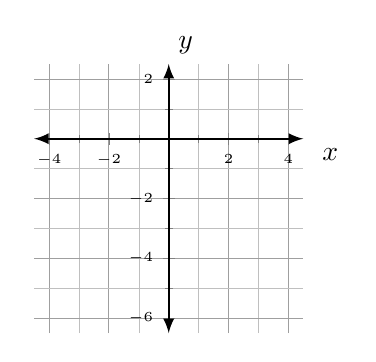
\begin{tikzpicture}[>=latex]
				\begin{axis}[
						    width =5cm,
					               height=5cm,
						    xmin=-4,xmax=4,
						    ymin=-6,ymax=2,
						    grid=both,
						    grid style={line width=.15pt, draw=gray!50},
						    major grid style={line width=.3pt,draw=gray!75},
						    axis lines=middle,
						    minor tick num=1,
						    enlargelimits={abs=0.5},
						    axis line style={latex-latex, thick},
						    ticklabel style={font=\tiny,fill=none},
						    xlabel={\,\,$x$},
						    ylabel={$y$},
						    xlabel style={below right},
						    ylabel style={above right}
						]
				\end{axis}
		\end{tikzpicture}
	\end{flushright}
\end{minipage}
\hspace{1cm}
\begin{minipage}{0.45\linewidth}
\vspace{-0.35cm}
	\begin{enumerate}
		%
		\vspace{1cm}
		%
		\setcounter{enumi}{1}
		\item
			$\begin{cases}
				x-3y=6\\
				3x-y=2
			\end{cases}$\\
	\end{enumerate}
	%
	\vspace{-2cm}
	%
	\begin{flushright}
		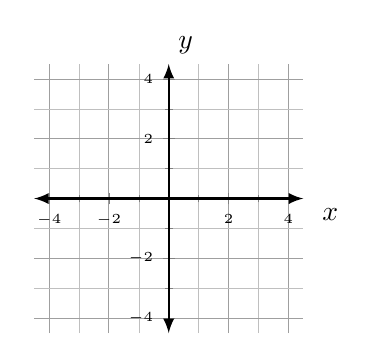
\begin{tikzpicture}[>=latex]
				\begin{axis}[
						    width =5cm,
					               height=5cm,
						    xmin=-4,xmax=4,
						    ymin=-4,ymax=4,
						    grid=both,
						    grid style={line width=.15pt, draw=gray!50},
						    major grid style={line width=.3pt,draw=gray!75},
						    axis lines=middle,
						    minor tick num=1,
						    enlargelimits={abs=0.5},
						    axis line style={latex-latex, thick},
						    ticklabel style={font=\tiny,fill=none},
						    xlabel={\,\,$x$},
						    ylabel={$y$},
						    xlabel style={below right},
						    ylabel style={above right}
						]
				\end{axis}
		\end{tikzpicture}
	\end{flushright}
\vspace{0.35cm}
\end{minipage}

%
\vspace{-1cm}
%

\noindent Classify each system and determine the number of solutions.\\

%
\vspace{-0.5cm}
%
\begin{minipage}{0.45\linewidth}
	\begin{enumerate}
		\setcounter{enumi}{2}
		\item 
			$\begin{cases}
				y=x-7\\
				x+9y=16
			\end{cases}$
	\end{enumerate}
	%
	\vspace{1cm}
	%
\end{minipage}
\hspace{1cm}
\begin{minipage}{0.45\linewidth}
	\begin{enumerate}
		\setcounter{enumi}{3}
		\item
			$\begin{cases}
				5x-10y=8\\
				x-2y=4
			\end{cases}$
	\end{enumerate}
	%
	\vspace{1cm}
	%

\end{minipage}\\

\noindent Use substitution or elimination to solve the following.\\

\vspace{-0.5cm}
\begin{minipage}{0.45\linewidth}
	\begin{enumerate}
		\setcounter{enumi}{4}
		\item
			$\begin{cases}
				y=3x\\
				2x-3y=-7
			\end{cases}$
		%
		\vspace{2cm}
		%
		\item
			$\begin{cases}
				-4x-y=-16\\
				-4x-5y=-32
			\end{cases}$
		%
		\vspace{1cm}
		%
	\end{enumerate}
\end{minipage}
\hspace{1cm}
\begin{minipage}{0.45\linewidth}
	\begin{enumerate}
		\setcounter{enumi}{6}
		\item
			$\begin{cases}
				4x+5y=41\\
				7x+5y=53
			\end{cases}$
		%
		\vspace{2cm}
		%
		\item
			$\begin{cases}
				9x-5y=13\\
				4x-6y=2
			\end{cases}$
		%
		\vspace{1cm}
		%
	\end{enumerate}
\end{minipage}\\


\begin{enumerate}
\setcounter{enumi}{8}
\item A popular mixture of potpourri includes pine needles and lavender. If pine needles cost $\$1.50$ per ounce and lavender costs $\$4.00$ per ounce, how much of each ingredient should be mixed to make 80 oz of potpurri worth $\$200.00$?
\end{enumerate}
\vspace{1.5cm}

\noindent Graph the system of inequalities.

\begin{minipage}{0.45\linewidth}
	%
	\vspace{-0.5cm}
	%
	\begin{enumerate}
		\setcounter{enumi}{9}
		\item
			$\begin{cases}
				y-1>4x\\
				y\leq x+1
			\end{cases}$\\
	\end{enumerate}
	%
	\vspace{-2cm}
	%
	\begin{flushright}
		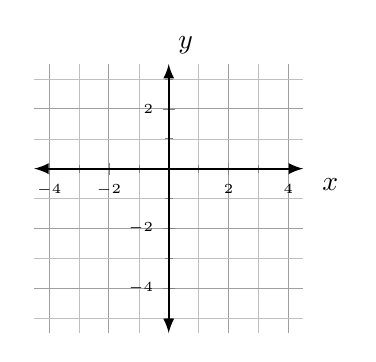
\begin{tikzpicture}[>=latex]
				\begin{axis}[
						    width =5cm,
					               height=5cm,
						    xmin=-4,xmax=4,
						    ymin=-5,ymax=3,
						    grid=both,
						    grid style={line width=.15pt, draw=gray!50},
						    major grid style={line width=.3pt,draw=gray!75},
						    axis lines=middle,
						    minor tick num=1,
						    enlargelimits={abs=0.5},
						    axis line style={latex-latex, thick},
						    ticklabel style={font=\tiny,fill=none},
						    xlabel={\,\,$x$},
						    ylabel={$y$},
						    xlabel style={below right},
						    ylabel style={above right}
						]
				\end{axis}
		\end{tikzpicture}
	\end{flushright}
\end{minipage}
\hspace{1cm}
\begin{minipage}{0.45\linewidth}
\vspace{-0.5cm}
	\begin{enumerate}
		\setcounter{enumi}{10}
		\item
			$\begin{cases}
				y\leq -x+2\\
				x>-1\\
				y>-1
			\end{cases}$\\
	\end{enumerate}
\vspace{-2.5cm}
	\begin{flushright}
		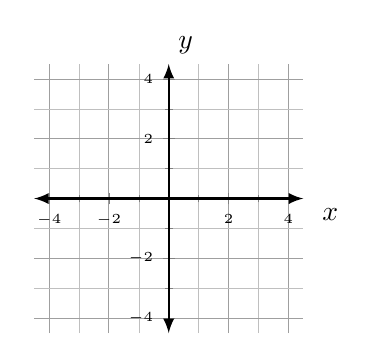
\begin{tikzpicture}[>=latex]
				\begin{axis}[
						    width =5cm,
					               height=5cm,
						    xmin=-4,xmax=4,
						    ymin=-4,ymax=4,
						    grid=both,
						    grid style={line width=.15pt, draw=gray!50},
						    major grid style={line width=.3pt,draw=gray!75},
						    axis lines=middle,
						    minor tick num=1,
						    enlargelimits={abs=0.5},
						    axis line style={latex-latex, thick},
						    ticklabel style={font=\tiny,fill=none},
						    xlabel={\,\,$x$},
						    ylabel={$y$},
						    xlabel style={below right},
						    ylabel style={above right}
						]
				\end{axis}
		\end{tikzpicture}
	\end{flushright}
\end{minipage}


\newpage

\begin{enumerate}
    \setcounter{enumi}{11}
    \item A coffee shop wants to make a maximum of 120 lbs of a coffee mixture that costs less than $\$10$/lb. The shop will mix coffee that is sold at $\$8$/lb with coffee sold at $\$11.50$/lb. Write and graph a system of inequalities that shows the possible mixtures of the two coffee types. 
    \vspace{2cm}
    \item\label{region} Graph the feasible region. 
    $\begin{cases}
    x\geq 0\\
    y \geq 0 \\
    y\leq 3x+1\\
    y\leq \displaystyle -\frac{3}{4}x+6
    \end{cases}
    $
    \vspace{-3.5cm}
    \begin{flushright}
                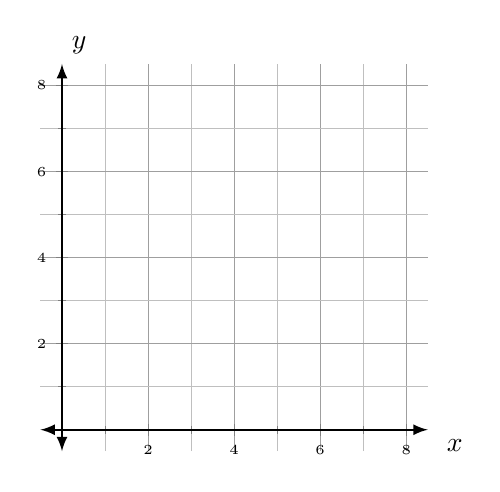
\begin{tikzpicture}[>=latex]
    				\begin{axis}[
    						    width =6.5cm,
    					        height=6.5cm,
    						    xmin=0,xmax=8,
    						    ymin=0,ymax=8,
    						    grid=both,
    						    grid style={line width=.15pt, draw=gray!50},
    						    major grid style={line width=.3pt,draw=gray!75},
    						    axis lines=middle,
    						    minor tick num=1,
    						    enlargelimits={abs=0.5},
    						    axis line style={latex-latex, thick},
    						    ticklabel style={font=\tiny,fill=none},
    						    xlabel={\,\,$x$},
    						    ylabel={$y$},
    						    xlabel style={below right},
    						    ylabel style={above right},
    						]
    				\end{axis}
    		    \end{tikzpicture}
    \end{flushright}
    \vspace{1cm}
    \item Maximize $P=6x+10y$ for the constraints in problem \ref{region}.
    \vspace{2cm}
    \item A shoe company produces two models of insoles: thick and thin. The thick insole requires 6 min of manufacturing time and generates a profit of $\$8$. The thin insole requires 4 min of manufacturing time and generates a profit of $\$9$. The line runs at most 12 hrs a day (720 min) Because of demand the company wants to produce at least twice as many thick insoles as thin insoles.
        \begin{itemize}
            
            \item[(a)] Write the constraints and graph the feasible region.
            \vspace{-1cm}
                \begin{flushright}
                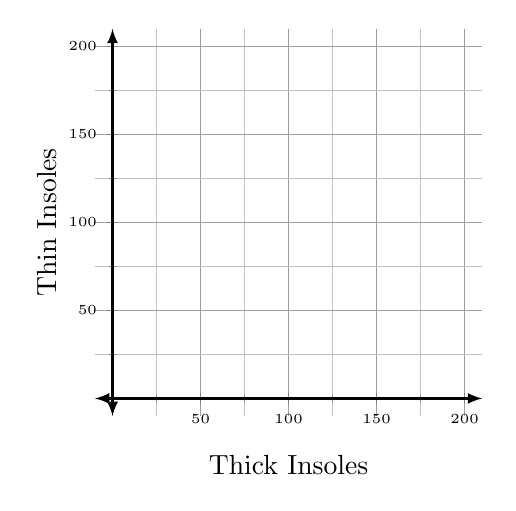
\begin{tikzpicture}[>=latex]
    				\begin{axis}[
    						    width =6.5cm,
    					        height=6.5cm,
    						    xmin=0,xmax=200,
    						    ymin=0,ymax=200,
    						    grid=both,
    						    grid style={line width=.15pt, draw=gray!50},
    						    major grid style={line width=.3pt,draw=gray!75},
    						    axis lines=middle,
    						    minor tick num=1,
    						    enlargelimits={abs=10},
    						    axis line style={latex-latex, thick},
    						    ticklabel style={font=\tiny,fill=none},
    						    xlabel={\,\,$x$},
    						    ylabel={$y$},
    						    xlabel style={below right},
    						    ylabel style={above right},
    						    xlabel={Thick Insoles},
				                ylabel={Thin Insoles},
				                x label style={at={(axis description cs:0.5,-0.075)},anchor=north},
				                y label style={at={(axis description cs:-0.075,.5)},rotate=90,anchor=south},
    						]
    				\end{axis}
    		    \end{tikzpicture}
    		  \end{flushright}
            \item[(b)] Write the objective function for the company's profit.
            \vspace{1cm}
            \item[(c)] What is the maximum profit that can be generated in one day?
            \vspace{3cm}
        \end{itemize}
\end{enumerate}

%%%%%%%%%%%%%%%%%%%%%%%%%%%%%%%%%%%%%%%%%%%%%%%%
%%%%%%%%%%%%%%%%%%%%%%%%%%%%%%%%%%%%%%%%%%%%%%%%
\newpage
%%%%%%%%%%%%%%%%%%%%%%%%%%%%%%%%%%%%%%%%%%%%%%%%
%%%%%%%%%%%%%%%%%%%%%%%%%%%%%%%%%%%%%%%%%%%%%%%%

\begin{enumerate}
    \setcounter{enumi}{15}
    \item Graph Each point in three dimensional space.\\
    
    \begin{minipage}{0.25\linewidth}
    \vspace{-3cm}
        $(a)$ $(-1,0,3)$\\
        
        $(b)$ $(2,-2,1)$\\
    \end{minipage}
    \begin{minipage}{0.25\linewidth}
    \vspace{-3cm}
        $(c)$ $(0,-1,1)$\\
        
        $(d)$ $(3,1,0)$\\
    \end{minipage}
    \begin{minipage}{0.45\linewidth}
        \vspace{-1.75cm}
            %%%%%%%%%%%%%%%%% 3space Axes to Plot On
            \begin{tikzpicture}[x=0.5cm,y=0.5cm,z=0.3cm,>=latex,scale=1.1]
                % The axes
                \draw[->] (xyz cs:x=-5.5) -- (xyz cs:x=5.5) node[above] {$y$};
                \draw[->] (xyz cs:y=-5.5) -- (xyz cs:y=5.5) node[right] {$z$};
                \draw[<-] (xyz cs:z=-5.5) node[above] {$x$} -- (xyz cs:z=5.5);
                % The thin ticks
                \foreach \coo in {-5,-4,...,5}
                {
                  \draw (\coo,-1.5pt) -- (\coo,1.5pt);
                  \draw (-1.5pt,\coo) -- (1.5pt,\coo);
                  \draw (xyz cs:y=-0.15pt,z=\coo) -- (xyz cs:y=0.15pt,z=\coo);
                }
                % The thick ticks
                \foreach \coo in {5,-5}
                {
                  \draw[thick] (\coo,-3pt)  node[below]{\coo} -- (\coo,3pt) ;
                  \draw[thick] (-3pt,\coo) -- (3pt,\coo) node[left=6pt] {\coo};
                  \draw[thick] (xyz cs:y=-0.3pt,z=-\coo) -- (xyz cs:y=0.3pt,z=-\coo) node[below=8pt] {\coo};
                }
            \end{tikzpicture}
            %%%%%%%%%%%%%%%%%
    \end{minipage}
    \vspace{-2cm}
    \item Use elimination to solve the system of equations.\\
    	$
    	\begin{cases}
    	x+3y+2z=13\\
    	2x+2y-z=3\\
    	x-2y+3z=6
    	\end{cases}
    	$
    \vspace{2cm}
    \item Classify the system as consistent or inconsistent and determine the number of solutions.\\
        $
    	\begin{cases}
    	x+y+z=-2\\
    	-x+2y-5z=4\\
    	3x+3y+3z=5
    	\end{cases}
    	$
    \vspace{1.5cm}
\end{enumerate}




\hrule
\color{red}
\noindent \underline{Solutions}:\\

\vspace{-1cm}
\begin{minipage}{0.3\linewidth}
    \begin{enumerate}
        \item $(5,10)$
        \item $(0,-2)$
        \item Consistent, One Solution
        \item Inconsistent, No Solution
        \item $(1,3)$
        \item $(3,4)$
        \item $(4,5)$
        \item $(2,1)$
        \item 48 oz pine, 32 oz of lavender
        \vspace{-0.25cm}
        \item 		
            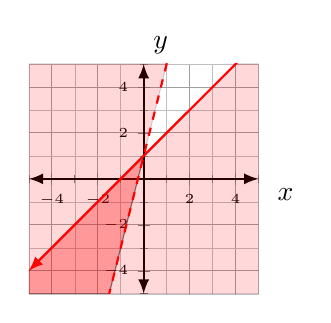
\begin{tikzpicture}[>=latex]
    				\begin{axis}[
    						    width =4.5cm,
    					        height=4.5cm,
    						    xmin=-4,xmax=4,
    						    ymin=-4,ymax=4,
    						    grid=both,
    						    grid style={line width=.15pt, draw=gray!50},
    						    major grid style={line width=.3pt,draw=gray!75},
    						    axis lines=middle,
    						    minor tick num=1,
    						    enlargelimits={abs=1},
    						    axis line style={latex-latex, thick},
    						    ticklabel style={font=\tiny,fill=none},
    						    xlabel={\,\,$x$},
    						    ylabel={$y$},
    						    xlabel style={below right},
    						    ylabel style={above right},
    						]
    				\draw [fill=red, opacity=0.4]
                    (0,1) -- (-1.5,-5) -- (-5,-5) -- (-5,-4)--cycle;
                    \draw [fill=red, opacity=0.15]
                    (0,1) -- (-1.5,-5) -- (5,-5) -- (5,5)--(4,5)--cycle;
                    \draw [fill=red, opacity=0.15]
                    (0,1) -- (1,5) -- (-5,5) -- (-5,-4)--cycle;
                    \addplot[<->, dashed ,red,thick,domain=-5:5] {4*x+1};
                    \addplot[<->,red,thick,domain=-5:5] {x+1};
    				\end{axis}
    		    \end{tikzpicture}
        \end{enumerate}
    \end{minipage}
    \begin{minipage}{0.3\linewidth}
        \begin{enumerate}
        \setcounter{enumi}{10}
    		    \item            
        		    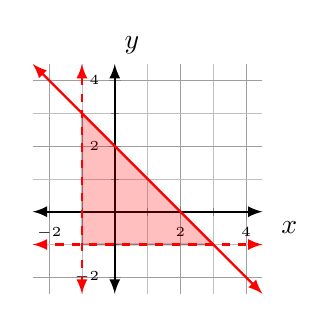
\begin{tikzpicture}[>=latex]
        				\begin{axis}[
        						    width =4.5cm,
        					        height=4.5cm,
        						    xmin=-2,xmax=4,
        						    ymin=-2,ymax=4,
        						    grid=both,
        						    grid style={line width=.15pt, draw=gray!50},
        						    major grid style={line width=.3pt,draw=gray!75},
        						    axis lines=middle,
        						    minor tick num=1,
        						    enlargelimits={abs=0.5},
        						    axis line style={latex-latex, thick},
        						    ticklabel style={font=\tiny,fill=none},
        						    xlabel={\,\,$x$},
        						    ylabel={$y$},
        						    xlabel style={below right},
        						    ylabel style={above right},
        						]
        				\draw [thick, draw=black, fill=red, opacity=0.25]
                        (-1,-1) -- (3,-1) -- (-1,3) -- cycle;
                        \addplot[<->,red,thick,domain=-2.5:4.5] {-1*x+2};
                        \addplot[<->,dashed,red,thick,domain=-2.5:4.5] {-1};
                        \draw[<->, dashed, red, thick] (-1,4.5) -- (-1,-2.5); 
        				\end{axis}
        		    \end{tikzpicture}
        \item 
            $
            \begin{cases}
            x+y\leq 120\\
            8x+11.5y<1200
            \end{cases}
            $
        \item 
            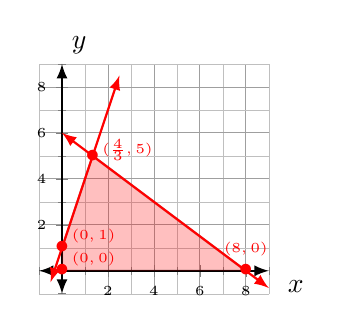
\begin{tikzpicture}[>=latex]
    				\begin{axis}[
    						    width =4.5cm,
    					        height=4.5cm,
    						    xmin=0,xmax=8,
    						    ymin=0,ymax=8,
    						    grid=both,
    						    grid style={line width=.15pt, draw=gray!50},
    						    major grid style={line width=.3pt,draw=gray!75},
    						    axis lines=middle,
    						    minor tick num=1,
    						    enlargelimits={abs=1},
    						    axis line style={latex-latex, thick},
    						    ticklabel style={font=\tiny,fill=none},
    						    xlabel={\,\,$x$},
    						    ylabel={$y$},
    						    xlabel style={below right},
    						    ylabel style={above right},
    						]
    				\draw [thick, draw=black, fill=red, opacity=0.25]
                    (0,0) -- (0,1) -- (4/3,5) -- (8,0)--cycle;
                    \addplot[<->,red,thick,domain=-0.5:2.5] {3*x+1};
                    \addplot[<->,red,thick,domain=0:9] {-3/4*x+6};
                    \node [red] at (4/3,5) {$\bullet$};
                    \node [red, right] at (4/3,5.25) {\tiny$(\frac{4}{3},5)$\normalsize};
                    \node [red] at (0,1) {$\bullet$};
                    \node [red, right] at (0,1.5) {\tiny$(0,1)$\normalsize};
                    \node [red] at (0,0) {$\bullet$};
                    \node [red, right] at (0,0.5) {\tiny$(0,0)$\normalsize};
                    \node [red] at (8,0) {$\bullet$};
                    \node [red,above] at (8,0.2) {\tiny$(8,0)$\normalsize};
    				\end{axis}
    		    \end{tikzpicture}
    	\item 58

    \end{enumerate}
\end{minipage}
\begin{minipage}{0.3\linewidth}
    \vspace{-0.5cm}
    \begin{enumerate}
        \setcounter{enumi}{14}
        \item
    	$(a)
    	\begin{cases}
    	x\geq 0\\
    	y\geq 0\\
    	6x+4y\leq 720\\
    	x\geq 2y
    	\end{cases}\\
    	$
    	            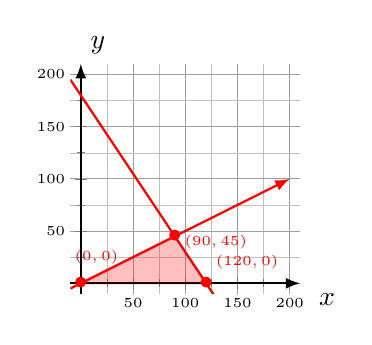
\begin{tikzpicture}[>=latex]
    				\begin{axis}[
    						    width =4.5cm,
    					        height=4.5cm,
    						    xmin=0,xmax=200,
    						    ymin=0,ymax=200,
    						    grid=both,
    						    grid style={line width=.15pt, draw=gray!50},
    						    major grid style={line width=.3pt,draw=gray!75},
    						    axis lines=middle,
    						    minor tick num=1,
    						    enlargelimits={abs=10},
    						    axis line style={-latex, thick},
    						    ticklabel style={font=\tiny,fill=none},
    						    xlabel={\,\,$x$},
    						    ylabel={$y$},
    						    xlabel style={below right},
    						    ylabel style={above right},
    						]
    				\draw [thick, draw=black, fill=red, opacity=0.25]
                    (0,0) -- (120,0) -- (90,45) --cycle;
                    \addplot[->,red,thick,domain=-10:200] {-1.5*x+180};
                    \addplot[->,red,thick,domain=-10:200] {0.5*x};
                    \node [red] at (90,45) {$\bullet$};
                    \node [red,right] at (90,40) {\tiny$(90,45)$\normalsize};
                    \node [red] at (120,0) {$\bullet$};
                    \node [red,right] at (120,20) {\tiny$(120,0)$\normalsize};
                    \node [red] at (0,0) {$\bullet$};
                    \node [red] at (15,25) {\tiny$(0,0)$\normalsize};
    				\end{axis}
    		    \end{tikzpicture}\\
    	$(b)$ $P=8x+9y$\\
    	$(c)$ $\$1125$
    \item
    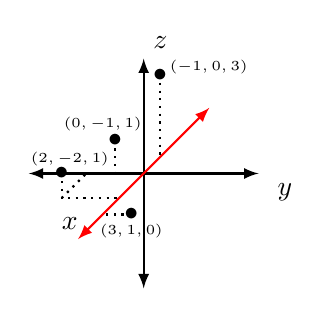
\begin{tikzpicture}[>=latex]
    				\begin{axis}[
    						    width =4.5cm,
    					        height=4.5cm,
    						    xmin=-6,xmax=6,
    						    ymin=-6,ymax=6,
    						    axis lines=middle,
    						    enlargelimits={abs=1},
    						    xtick style = {draw=none},
    						    ytick style = {draw=none},
    						    xticklabels={,,},
    						    yticklabels={,,},
    						    axis line style={latex-latex, thick},
    						    xlabel={\,\,$y$},
    						    ylabel={$z$},
    						    xlabel style={below right},
    						    ylabel style={above right},
    						]
                    \addplot[<->,red,thick,domain=-4:4] {x};
                    \node[above] at (-4.5,-4) {$x$};
                    \node at (-0.75,-2.5) {$\bullet$};
                    \node[below] at (-0.75,-2.5) {\tiny$(3,1,0)$\normalsize};
                    \draw[dotted,thick] (-0.75,-2.5) -- (-2.5,-2.5);
                    \node at (-5,0) {$\bullet$};
                    \node[above] at (-4.5,-0.15) {\tiny$(2,-2,1)$\normalsize};
                    \draw[dotted,thick] (-5,0) -- (-5,-1.5)--(-1.5,-1.5);
                    \draw[dotted,thick] (-5,-1.5)--(-3.5,0);
                    \node at (-1.75,2) {$\bullet$};
                    \node[above] at (-2.5,2) {\tiny$(0,-1,1)$\normalsize};
                    \draw[dotted,thick] (-1.75,2)--(-1.75,0);
                    \node at (1,6) {$\bullet$};
                    \node[right] at (1,6.5) {\tiny$(-1,0,3)$\normalsize};
                    \draw[dotted,thick] (1,6)--(1,1);
    				\end{axis}
    		    \end{tikzpicture}
        \item $(1,2,3)$
        \item inconsistent, no solution
    \end{enumerate}
\end{minipage}




%\begin{minipage}{0.45\linewidth}
%	\begin{enumerate}
%		\setcounter{enumi}{0}
%		\item 
%		\item
%		\item
%		\item
%		\item
%	\end{enumerate}
%\end{minipage}
%\hspace{1cm}
%\begin{minipage}{0.45\linewidth}
%	\begin{enumerate}
%		\setcounter{enumi}{0}
%		\item
%		\item
%		\item
%		\item
%		\item
%	\end{enumerate}
%\end{minipage}\\



\end{document}










